\documentclass{article}

\usepackage{xcolor}
\usepackage{tcolorbox}     % Color boxes
\usepackage{amsmath}       % Basic mathematical typesetting
\usepackage{amssymb}       % Advanced math symbols
\usepackage{amsthm}        % Theorems typesetting
\usepackage{array}         % Advanced table column formats
\usepackage{enumitem}      % Itemize/enumrate
\usepackage{fancyhdr}      % Custom header/footer styles
\usepackage{fourier}       % Adobe Utopia font
\usepackage{graphicx}      % Enhanced images support
\usepackage{ifluatex}      % LuaTeX-specific options
\usepackage{kantlipsum}    % English kantian-style lipsum
\usepackage{lipsum}        % Lorem ipsum
\usepackage{listings}      % Code listings
\usepackage{longtable}     % Multi-page tables
\usepackage{multirow}      % Advanced table cells
\usepackage{setspace}      % Set space between lines
\usepackage{scrextend}     % Allows \addmargin environment
\usepackage{tablefootnote} % Table footnotes
\usepackage{tocloft}       % Custom ToC/LoF/LoT
\usepackage{url}           % URL-sensitive line breaks
\usepackage{xspace}        % Remove duplicated spaces

\setstretch{1.15}
\setlength{\parindent}{5mm}
\counterwithin{equation}{section}
\counterwithin{figure}{section}
\counterwithin{table}{section}
\setcounter{tocdepth}{3}
\setcounter{secnumdepth}{3}

% List formatting
\setlist[itemize,1]{topsep=2pt,label=\large$\bullet$, leftmargin=28pt}
\setlist[itemize,2]{topsep=2pt,leftmargin=18pt}
\setlist[itemize,3]{topsep=2pt,leftmargin=18pt}
\setlist[enumerate,1]{topsep=2pt,leftmargin=24pt}
\setlist[enumerate,2]{topsep=2pt,leftmargin=16pt}
\setlist[enumerate,3]{topsep=2pt,leftmargin=16pt}

% List of figures
\renewcommand*\l@figure{\@dottedtocline{1}{0.5em}{2.25em}}
\newcommand{\listoffigurestoc}{
    \listoffigures
    \addcontentsline{toc}{section}{\listfigurename}
}

% List of tables
\renewcommand*\l@table{\@dottedtocline{1}{0.5em}{2.25em}}
\newcommand{\listoftablestoc}{
    \listoftables
    \addcontentsline{toc}{section}{\listtablename}
}

% region LuaLatex Scripts

% Script from: https://github.com/ArturB/WUT-Thesis
\usepackage{ifluatex}      % LuaTeX-specific options
\ifluatex
    \usepackage[T1]{fontenc}
    \usepackage[utf8]{luainputenc}
    \usepackage{luacode}
    % In LuaTeX, we can prevent one-letter words
    % from beging at the end of the line.
    \begin{luacode}
    local debug = false
    local glyph_id = node.id "glyph"
    local glue_id  = node.id "glue"
    local hlist_id = node.id "hlist"

    local prevent_single_letter = function (head)
        while head do
            if head.id == glyph_id then
                if unicode.utf8.match(unicode.utf8.char(head.char),"%a") then     -- is a letter
                    if head.prev.id == glue_id and head.next.id == glue_id then   -- is one letter word

                        local p = node.new("penalty")
                        p.penalty = 10000

                        if debug then
                            local w = node.new("whatsit","pdf_literal")
                            w.data = "q 1 0 1 RG 1 0 1 rg 0 0 m 0 5 l 2 5 l 2 0 l b Q"
                            node.insert_after(head,head,w)
                            node.insert_after(head,w,p)
                        else
                            node.insert_after(head,head,p)
                        end
                    end
                end
            end
            head = head.next
        end
        return true
    end

    luatexbase.add_to_callback("pre_linebreak_filter",prevent_single_letter,"~")
    \end{luacode}
\fi

% endregion

% region Custom Tags

\newcommand{\temporary}[1]{
    \begin{tcolorbox}[colframe=red, colback=white, title={\textbf{WERSJA PO POLSKU}}, sharp corners=south]
        #1
    \end{tcolorbox}
}

% endregion

\begin{document}

    \title{Title of article}
    \author{Patryk Filip Gryz}

    \maketitle

    \clearpage
    \section{Introduction}

        \subsection{Background}

            \temporary{
                Odkrycie DNA zapoczątkowało nową erę w biologii oraz medycynie, umożliwiając badania nad molekularnymi podstawami życia oraz precyzyjną diagnostykę wielu chorób\cite{Louie:2000}. Pierwsze kroki na tej drodze uczynił w 1869 roku Friedrich Miescher, który po raz pierwszy wyizolował z jądra komórkowego substancję nazwaną przez niego ,,nukleiną''\cite{Dahm:2005}, później zidentyfikowaną jako kwas deoksyrybonukleinowy. W latach 1895 - 1901 Albrecht Kossel wyizolował oraz nazwał cztery podstawowe zasady azotowe budujące kwas deoksyrybonukleinowy — adeninę, tyminę, cytozynę oraz guaninę\cite{Kossel:1893}. Przełomowe znaczenie DNA w przenoszeniu informacji genetycznej wykazano jednak dopiero w 1944 roku dzięki eksperymentowi Avery'ego-MacLeoda-McCarty'ego\cite{Avery:1944}, w którym udowodnili, że to DNA, a nie białka są nośnikiem informacji. W 1951 Erwin Chargaff odkrył prawidłowość, że ilość adeniny w DNA jest porównywalna do ilości tyminy, a ilość guaniny do ilości cytozyny\cite{Chargaff:1952}. Prawidłowość ta, nazwa później na cześć odkrywcy zasadami Chargaffa, stała się jedną z kluczowych przesłanek do odkrycia struktury podwójnej helisy DNA przez Watsona i Cricka w 1953 roku\cite{Watson:1953}.

    W 1970 Francis Crick sformułował centralny dogmat biologii molekularnej\cite{Crick:1970}, który głosi, że informacja genetyczna przepływa z DNA do RNA, a następnie do białek tworząc fundament współczesnej biologii molekularnej. Dalsze przełomowe odkrycia metod sekwencjonowania, opracowane w 1976 roku przez Allana Maxima oraz Waltera Gilberta\cite{Maxam:1977}, a także w 1977 roku przez Fredericka Sangera\cite{Sanger:1977}, pozwoliły na odczytywanie sekwencji DNA dowolnych organizmów, otwierając nowe możliwości badań nad DNA oraz przepływem informacji genetycznej. W tym samym czasie zespołowi Fredericka Sangera za pomocą nowej metody udało się po raz pierwszy przeprowadzić sekwencjonowanie całości materiału genetycznego  wirusa DNA — bakteriofaga $\phi{}$X174\cite{Sanger:1977:2}. Odkrycie to uwypukliło ograniczenia tradycyjnych metod analizy i wykazało konieczność zastosowania komputerów do przetwarzania sekwencji DNA\cite{Staden:1979}.

    W miarę postępu badań nad sekwencjami DNA, zespoły badawcze rozpoczęły gromadzenie sekwencji, w celu dalszych analiz i porównań. Pod koniec lat 70. XX wieku pojawiła się potrzeba stworzenia bazy danych, która umożliwiałaby gromadzenie sekwencji w celu ich późniejszego wykorzystania oraz redukcji kosztów badań. Odpowiedzią na to zapotrzebowanie było sfinansowanie bazy danych ,,GenBank'' w 1982 roku w Stanach Zjednoczonych\cite{Bilofsky:1986} oraz europejskiej bazy danych ,,EBML Data Library'' w 1980 roku\cite{Higgins:1992}. W 1983 roku Johnowi Wilburowi oraz Davidowi Lipmanowi udało się opracować algorytm wyszukiwania sekwencji podobnych w bazach danych\cite{Wilbur:1983}, co pozwoliło na szybkie porównywanie sekwencji genetycznych. W 1990 roku wprowadzono narzędzie BLAST\cite{Altschul:1990}, które przyśpieszyło ten proces.

    Pierwszy pomysł analizy materiału genetycznego wielu organizmów jednocześnie bez konieczności ich hodowli został zaproponowany w 1998 roku przez Jo Handlesmana i jego zespół\cite{Handelsman:1998}. Zespół badał organizmy obecne w glebie. Wykorzystanie informacji o materiale genetycznym znalezionym w środowisku, w połączeniu z bazami danych sekwencji, umożliwia  identyfikację organizmów obecnych w badanej próbce. Proces analizy dużej liczby sekwencji DNA oraz ich porównywanie z bazami danych wymaga jednak znacznych zasobów obliczeniowych.

    Wraz z rozwojem metod sekwencjonowania nowej generacji\cite{Reinartz:2002}, koszty sekwencjonowania znacząco spadły, a liczba analizowanych sekwencji DNA znacznie wzrosła\cite{Muir:2016}. Dalsze gromadzenie danych sekwencyjnych oraz wzrost przepustowości technologii sekwencjonowania prowadzą do zwiększonego zapotrzebowania na zasoby obliczeniowe.
            }
        
        \subsection{Motivation}

            The time required for taxonomic classification of large sequence datasets using traditional tools, such as BLAST, can span several hours, even for relatively small collections of sequences e.g. 4096 sequences. In many fields, artificial neural networks (ANN) have demonstrated the ability to outperform classical heuristic algorithms, offering faster and more accurate results. By leveraging the capabilities of ANN, this works aims to accelerate taxonomic clasisfication process while maintaining at least the same level of quality as traditional methods.

        \subsection{Objectives}
    
            The primary objective of this study is to leverage an artificial neural network to support the selection of representative genetic sequences for taxonomic classification. Instead of classifying entire environmental genetic sequences sample, the proposed approach focuses on identifying a subset of sequences that best represent the sample. These selected representatives are then classified, reducing computational complexity while maintaining classification accuracy.

        \subsection{Main Contributions}

            This paper introduces a novel artificial neural network model for calculating dissimilarities between genetic sequences, which can be used in clustering algorithm to select representative sequences for taxonomic classification. We provide all the necessary components for training the model, including dataset preparation, batch process, a loss function, and a training loop. The paper also includes an application that can perform taxonomic classification with specified parameters. Furthermore, we develope a library that allows users to compose the taxonomic classification pipelines.

        \subsection{Structure of the Paper}

            The rest of the paper is organized as follows. Section 2 provides a description of related work, reviewing previous research on taxonomic classification and highlights a research gap. Section 3 defines the problem, presents the proposed approach, and provides detailed implementation details. Section 4 describes the experimental setup, including used datasets, the performance metrics for evaluation, and the results obtained from experiments with analysis. Section 5 interprets the results, discusses the limtiations of proposed approach, and explores possible improvements for future work. Finally, Section 6 concludes the paper by summarizing the main findings and suggesting potential directions for future research.

    \clearpage
    \section{Related Work}

        \subsection{Overview of Existing Approaches}

            \temporary{
                Badania nad klasyfikacją taksonomiczną sekwencji DNA cechują się dynamicznym rozwojem w ciągu ostatnich 25 lat. Wprowadzenie metod sekwencjonowania nowej generacji pozwoliło na analizę dużych ilości materiału genetycznego pochodzącego z różnych środowisk. Optymalizacja procesu klasyfikacji taksonomicznej stała się głównym kierunkiem rozwoju narzędzi do klasyfikacji, szczególnie w przypadku narzędzi opartych na bazach danych sekwencji genetycznych, ponieważ liczba sekwencji w tych bazach podwaja się średnio co 30 miesięcy~\cite{Benson:2008}.

        Historycznie jednym z pierwszych algorytmów, który umożliwił klasyfikację taksonomiczną był algorytm Needlemana-Wunscha\cite{Needleman:1970} opracowany w 1970 roku, który pozwalał na porównywanie sekwencji genetycznych. Jednak pierwszym rozwiązaniem, które pozwalało na klasyfikację taksonomiczną w rozsądnym czasie, było narzędzie stworzone w 1983 roku przez D. Lipmana i W. Wilbura\cite{Wilbur:1983}. Bazowało ono na podziale sekwencji na $k$-krotki, które są uogólnieniem $k$-merów i ich porównywaniu. Rozwinięciem tego rozwiązania był algorytm ,,BLAST'' przedstawiony w 1990 roku\cite{Altschul:1990} bazujący na $k$-merach oraz umożliwiający wyszukiwanie sekwencji podobnych w bazach NCBI. Innym podejściem powstałym w podobnym okresie było narzędzie ,,Clustal''\cite{Higgins:1988} stworzone w 1988 roku, które pozwalało na wyrównywanie wielu sekwencji genetycznych.

        Największy postęp w badaniach nastąpił jednak w ciągu ostatnich 15 lat, czego przykładem jest utworzenie w 2012 roku narzędzia ,,MetaPhlAn''\cite{Segata:2012}, które wykorzystuje geny wskaźnikowe do porównywania składu gatunkowego próbek metagenomicznych. Kolejnym podejściem opartym na genach wskaźnikowych jest narzędzie ,,mOTUs2''\cite{Milanese:2019}, które bazuje na identyfikacji i analizie markerów unikalnych dla specyficznych szczepów mikroorganizmów. Inne podejście zostało zastosowane w narzędziu ,,Centrifuge''\cite{Kim:2016} opracowanym w 2016 roku, które wykorzystuje indeksowanie sekwencji za pomocą transformacji Burrowsa-Wheelera\cite{Burrows:1994} oraz indeksu Ferraginy-Manziniego\cite{Ferragina:2000} w celu efektywne wyszukiwania sekwencji podobnych. Bardziej klasyczne podejście zostało zastosowane w narzędziu ,,Kraken''\cite{Wood:2014} przedstawionym w 2014 roku, które wykorzystuje $k$-mery wraz z indeksowaną bazą sekwencji.

        Inną metodę optymalizacji procesu klasyfikacji taksonomicznej przedstawili Gautier i Lund w 2013 roku\cite{Gautier:2013}. Ich metoda opierała się na rozproszonej architekturze, w której serwer zwracał wskazówki dotyczące możliwych sekwencji do analizy na podstawie losowo wybranych sekwencji wejściowych, co pozwoliło na redukcję przesyłanych danych przez sieć. Nietypowe podejście do zadania klasyfikacji taksonomicznej przedstawiono w 2022 roku w narzędziu ,,BERTax''\cite{Mock:2022}. Narzędzie to wykorzystuje model typu transformer\cite{Transformers} do analizy sekwencji DNA, traktując je jako specyficzny język, na podstawie którego można dokonać przypisania bez potrzeby korzystania z baz referencyjnych. Kolejnym rozwiązaniem wykorzystującym modele uczenia maszynowego jest narzędzie ,,CGRclust''\cite{Alipour:2024}, które grupuje sekwencje DNA za pomocą dwuwymiarowej reprezentacji gier chaosu, łącząc nienadzorowane uczenie kontrastowe ze splotowymi sieciami neuronowymi.
            }

        \subsection{Comparatie Analysis}

            \temporary{
                Algorytmy bazujące na jakości wyrównania dają dobre wyniki, ale działają bardzo wolno.
                Algorytmy bazujące na $k$-merach działają szybko, ale nie uwzgledniają ukrytych wzorów w sekwencjach genetycznych
            }

        \subsection{Research Gaps}

            \temporary{
                Choć w ostatnich latach pojawiły się badania dotyczące klasyfikacji taksonomicznej z wykorzystaniem metod uczenia maszynowego, to wciąż brakuje prac skupiających się na zastosowaniu sztucznych sieci neuronowych z uczeniem kontrastowym do efektywnego grupowania sekwencji, co mogłoby znacząco przyspieszyć proces klasyfikacji przy użyciu dostępnych narzędzi.
            }

    \clearpage
    \section{Methodology}

        \subsection{Problem Definition}

            \temporary{
                Klasyfikacja taksonomiczna:

                Dla zbioru sekwencji A, szukamy takiego zbioru organizmów, że 

                \[
                    \forall a \in A \exists b \in B \text{ takie, że } a \text{ jest lokalnie podobne do } b_{sequence}
                \]
            }

        \subsection{Proposed Approach / Algorithm / Model}

            \temporary{
                W pracy zostaną wykorzystane dwa klasyczne podejścia do klasyfikacji taksonomicznej sekwencji genetycznych. Pierwsze z nich opiera się na wyrównaniu sekwencji, przy czym zostanie wykorzystany zmodyfikowany algorytm Needlemana-Wunscha. Drugie podejście wykorzystuje $k$-mery, w którym do obliczeń zostana zastosowane proste zanurzenia oraz odległość euklidesowa.

                \subsubsection{Algorytm Needlemana-Wunscha}
        
                    Algorytm Needlemana-Wunscha jest klasycznym algorytmem do wyrównywania globalnego sekwencji genetycznych. Metoda ta polega na zbudowaniu macierzy podobieństwa między sekwencjami zgodnie z ustalonymi regułami, które zostały przedstawione w równaniu~\eqref{Equation:NeedlemanWunsch}. W przypadku klasyfikacji taksonomicznej do dalszych obliczeń wystarczy wartość jakości dopasowania zawarta w $D_{n + 1, m + 1}$.
        
                    \begin{equation}
                        \begin{aligned}
                            D_{i,0} &= i \cdot g, & \text{dla } & i \in [1, n + 1] \\
                            D_{0,j} &= j \cdot g, & \text{dla } & j \in [2, m + 1] \\
                            D_{i,j} &= \max
                            \begin{cases}
                                D_{i - 1, j} + g \\
                                D_{i, j - 1} + g \\
                                D_{i - 1, j - 1} + s(A_i, B_j)
                            \end{cases}, & \text{dla } & i \in (1, n + 1] \text{ oraz } j \in (1, m + 1]
                        \end{aligned}
                        \label{Equation:NeedlemanWunsch}
                    \end{equation}
        
                    gdzie:
                    \begin{align*}
                        A, B -& \text{porównywane sekwencje}, \\
                        n, m -& \text{długości sekwencji } A \text{ oraz } B, \\
                        D -& \text{macierz podobieństwa o rozmiarach } n + 1 \text{ x } m + 1, \\
                        g \in \mathbb{R} -& \text{kara za przerwę}, \\
                        s(A_i, B_j) \in \mathbb{R} -& \text{podobieństwo między } i \text{-tym elementem w sekwencji A,} \\
                        & \text{a } j \text{-tym elementem w sekwencji B}. \\
                    \end{align*}
        
                \subsubsection{Zanurzenia $k$-merów}
        
                    Wykorzystanie $k$-merów w roli zanurzeń pozwala na reprezentację sekwencji DNA w postaci wektorów liczbowych, które można porównywać za pomocą różnych miar, takich jak na przykład odległość euklidesowa. Wektory liczbowe pozwalają na kompaktową reprezentację długich sekwencji, co znacznie przyśpiesza procesy grupowania sekwencji oraz klasyfikacji taksonomicznej. Metoda ta jest obecnie jedną z najpopularniejszych metod stosowanych do klasyfikacji taksonomicznej z wykorzystaniem baz danych, ponieważ cechuje się wysoką prędkością działania oraz pozwala uzyskać dobre wyniki. Obecne narzędzia wykorzystują różne miary, parametry $k$ oraz dodatkowe mechanizmy do dalszej optymalizacji tej metody.

                    \subsubsection{Sztuczna sieć neuronowa}

            Nową zaproponowaną metodą jest wykorzystanie sztucznej sieci neuronowej do redukcji wymiarowości wejściowych sekwencji DNA do postaci wektora cech o wymiarze $\mathbb{R}^{64}$. Sztuczna sieć neuronowa wykorzystuje uczenie kontrastowe, które umożliwia naukę reprezentacji danych wejściowych z zachowaniem własności podobieństwa oraz niepodobieństwa między wejściowymi sekwencjami. Niepodobieństwo między sekwencjami zostanie obliczone poprzez obliczenie niepodobieństwa kosinusowego wyrażonego wzorem~\eqref{Equation:CosineDissimilarity} między wektorami cech sekwencji DNA.

            \paragraph{Architektura}
                Architektura modelu sztucznej sieci neuronowej składa się z dwóch bloków splotowych oraz bloku perceptronów wielowarstwowych. Każdy z bloków splotowych zawiera warstwę splotową oraz warstwę normalizacji wsadowej i jest odpowiedzialny za ekstrakcję niskopoziomowych cech sekwencji. Ostatni blok splotowy jest połączony z blokiem perceptronów wielowarstwowych za pomocą warstwy spłaszczającej. Blok perceptronów wielowarstwowych odpowiada za tworzenie reprezentacji sekwencji, składa się z trzech warstw, które wykorzystują funkcję aktywacji GELU\cite{Hendrycks:2016}, z wyjątkiem ostatniej warstwy. Wyjściem całego modelu jest wektor cech o wymiarze $\mathbb{R}^{64}$.

                Schematycznie architektura została przedstawiona na rysunku~\ref{Picture:NeuralModel}.

                \begin{figure}[!htb]
                    \begin{center}
                        {
                        % ===== BEGIN =====
                        % ----- -----
                        % COLORS
                        % ----- -----
                        \definecolor{Green}{HTML}{1dd1a1}   % Input
                        \definecolor{Blue}{HTML}{54a0ff}    % Linear
                        \definecolor{Yellow}{HTML}{feca57}  % Convolution
                        \definecolor{Purple}{HTML}{5f27cd}  % Batch Norm
                        \definecolor{Grey}{HTML}{576574}    % Dropout
                        \definecolor{Red}{HTML}{ff6b6b}     % Output
                        \definecolor{Pink}{HTML}{ff9ff3}    % Activation
                        \definecolor{Background}{HTML}{c8d6e5}

                        % ----- -----
                        % ELEMENTS
                        % ----- -----
                        \tikzstyle{box} = [rectangle, rounded corners, minimum width=5cm, minimum height=1cm, text centered, draw=black, align=center]
                        \tikzstyle{input} = [box, fill=Green!30]
                        \tikzstyle{linear} = [box, fill=Blue!30]
                        \tikzstyle{conv} = [box, fill=Yellow!30]
                        \tikzstyle{bn} = [box, fill=Purple!30]
                        \tikzstyle{activation} = [box, fill=Pink!30]
                        \tikzstyle{dropout} = [box, fill=Grey!30]
                        \tikzstyle{output} = [box, fill=Red!30]

                        \tikzstyle{arrow} = [very thick, -Triangle]
                        \tikzstyle{arrow:text} = [pos=0.5, right, font=\footnotesize]

                        % ----- -----
                        % PICTURE
                        % ----- -----
                        \begin{tikzpicture}[node distance=2cm]
                            \node (input) [input] { Wejście };
                            \node (conv1) [conv, below of=input] { Splot 1D \\ \textbf{16@1x16, krok: 4} };
                            \node (bn1) [bn, below of=conv1] { Normalizacja wsadowa };
                            \node (conv2) [conv, below of=bn1] { Splot 1D \\ \textbf{32@1x8} };
                            \node (bn2) [bn, below of=conv2] { Normalizacja wsadowa };
                            \node (flatten) [linear, below of=bn2] { Warstwa spłaszczająca };
                            \node (flatten-right) [right of=flatten, xshift=2cm] {};

                            \node (fc1-left) [right of=input, xshift=2cm] {};
                            \node (fc1) [linear, right of=input, xshift=6cm] { Warstwa gęsta };
                            \node (act1) [activation, below of=fc1] { Aktywacja \\ \textbf{GELU} };
                            \node (drop1) [dropout, below of=act1] { Wyłączenie neuronów };
                            \node (fc2) [linear, below of=drop1] { Warstwa gęsta };
                            \node (act2) [activation, below of=fc2] { Aktywacja \\ \textbf{GELU} };
                            \node (drop2) [dropout, below of=act2] { Wyłączenie neuronów };
                            \node (fc3) [linear, below of=drop2] { Warstwa gęsta };
                            \node (output) [output, below of=fc3] { Wyjście };

                            \draw [arrow] (input) -- (conv1) node [arrow:text] {1x600};
                            \draw [arrow] (conv1) -- (bn1) node [arrow:text] {16x147};
                            \draw [arrow] (bn1) -- (conv2) node [arrow:text] {16x147};
                            \draw [arrow] (conv2) -- (bn2) node [arrow:text] {32x140};
                            \draw [arrow] (bn2) -- (flatten) node [arrow:text] {32x140};

                            \draw [arrow] (flatten.east) -- (flatten-right) -- node [arrow:text] {1x4480} (fc1-left) -- (fc1.west);
                            \draw [arrow] (fc1) -- (act1) node [arrow:text] {1x4096};
                            \draw [arrow] (act1) -- (drop1) node [arrow:text] {1x4096};
                            \draw [arrow] (drop1) -- (fc2) node [arrow:text] {1x4096};
                            \draw [arrow] (fc2) -- (act2) node [arrow:text] {1x512};
                            \draw [arrow] (act2) -- (drop2) node [arrow:text] {1x512};
                            \draw [arrow] (drop2) -- (fc3) node [arrow:text] {1x512};
                            \draw [arrow] (fc3) -- (output) node [arrow:text] {1x64};
                        \end{tikzpicture}

                        % ===== END =====
                        }
                    \end{center}
                    \caption{
                        Schemat architektury sieci neuronowej.
                    }\label{Picture:NeuralModel}
                \end{figure}

            \paragraph{Dane wejściowe}
                Wejściem modelu są sekwencje DNA o długości $150$, które są zakodowane do postaci wektora o wymiarach $1$ x $600$ za pomocą kodu 1 z n\cite{HarrisDavid:2007}.

            \paragraph{Przykłady uczące}
                Przykłady uczące oraz walidacyjne składają się z kotwicy (ang. \textit{anchor}), sekwencji pozytywnej (ang. \textit{positive}), czyli podobnej do kotwicy oraz sekwencji negatywnej (ang. \textit{negative}) niepodobnej do kotwicy.

            \paragraph{Zbiór danych}
                Zbiór danych uczących oraz walidacyjnych został stworzony na podstawie pierwszej próbki sekwencji genetycznych ze zbioru \textit{CAMI II Toy Human Microbiome Project}\cite{Fritz:2019}. Próbka zawiera symulowane dane metagenomiczne z mikrobiomu skóry człowieka. Przykłady zostały uzyskane poprzez losowanie kotwic ze zbioru oraz modyfikację tych kotwic w celu stworzenia sekwencji pozytywnej i negatywnej. Modyfikacja polegała na zamianie punktowej danego nukleotydu na inny. W przypadku sekwencji pozytywnej zmiana obejmowała od $0\%$ do $20\%$ długości kotwicy, natomiast w przypadku sekwencji negatywnej od $20\%$ do $80\%$ długości kotwicy.

            \paragraph{Funkcja straty}
                Wykorzystano funkcję straty zdefiniowaną jako:

                \begin{equation}
                    \text{Strata kontrastowa} = [m_{pos} - s_{pos}]_{+} + [s_{neg} - m_{neg}]_{+}
                \end{equation}

                gdzie:
                \begin{align*}
                    m_{pos} &- \text{margines podobieństwa między sekwencją pozytywną a kotwicą,} \\
                    m_{neg} &- \text{margines podobieństwa między sekwencją negatywną a kotwicą,} \\
                    s_{pos} &- \text{podobieństwo kosinusowe sekwencji pozytywnej do kotwic,} \\
                    s_{pos} &- \text{podobieństwo kosinusowe sekwencji negatywnej do kotwic.} \\
                \end{align*}

            \paragraph{Proces uczenia}
                Proces uczenia modelu sieci neuronowej został przeprowadzony na zbiorze $10^{6}$ przykładów uczących oraz $10^{4}$ przykładów walidacyjnych.
                W procesie wykorzystano optymalizator \textit{AdamW}\cite{Loshchilov2017DecoupledWD} z wykładniczym spadkiem współczynnika uczenia oraz zanikiem wag (ang. \textit{weight decay}).

            \paragraph{Miara jakości}
                Jako miarę jakości modelu wykorzystano stratę kontrastową modelu obliczoną na zbiorze walidacyjnym.

            \paragraph{Parametry procesu uczenia}
                Przeprowadzono eksperymenty w celu określenia optymalnych parametrów uczenia modelu sztucznej sieci neuronowej. Sprawdzono parametry współczynnika uczenia $\lambda$, zaniku wag $w$, współczynnika $\gamma$ stosowanego w wykładniczym spadku współczynnika uczenia, parametr wyłączania neuronów oraz stosowność trzech warstw perceptronów. W wyniku eksperymentów wybrano najlepsze parametry: $\lambda = 10^{-6}$, $w = $, $\gamma=0.99999$, współczynnik wyłączenia neuronów na poziomie $0.5$ oraz stwierdzono pozytywny wpływ zastosowania trzech warstw perceptronów.
                Wykorzystano również funkcję straty z parametrami: $m_{pos} = 1.0$, $m_{neg} = 0.25$.

            \paragraph{Wyniki procesu uczenia}

                W wyniku procesu uczenia modelu sztucznej sieci neuronowej, po 3 epokach uzyskano model, który osiągnął stratę równą $0.117$ na zbiorze walidacyjnym. Liczba epok została wybrana na podstawie analizy procesu uczenia, w którym po tej liczbie epok zaobserwowano nadmierne dopasowywanie się modelu (ang. \textit{overfitting}).


            Pełne wykorzystanie sztucznej sieci neuronowej w grupowaniu sekwencji zostało przedstawione na rysunku~\ref{Picture:Cluster:Neural}. Czerwonym obramowaniem oznaczono element wykorzystujący sztuczną sieć neuronową.

            \begin{figure}[!htb]
                \begin{center}
                    {
                    % ===== BEGIN =====
                    % ----- -----
                    % COLORS
                    % ----- -----
                    \definecolor{Green}{HTML}{1dd1a1}
                    \definecolor{Blue}{HTML}{54a0ff}
                    \definecolor{Yellow}{HTML}{feca57}
                    \definecolor{Purple}{HTML}{5f27cd}
                    \definecolor{Grey}{HTML}{576574}
                    \definecolor{Red}{HTML}{ff6b6b}
                    \definecolor{Pink}{HTML}{ff9ff3}
                    \definecolor{Background}{HTML}{c8d6e5}

                    % ----- -----
                    % ELEMENTS
                    % ----- -----
                    \tikzstyle{Circle} = [circle, minimum size=1cm, line width=2pt, draw=black]
                    \tikzstyle{Box} = [rectangle, minimum width=10cm, minimum height=1.5cm, line width=2pt, text centered, inner sep=10pt, draw=black]
                    \tikzstyle{Arrow} = [very thick, -Triangle]
                    \tikzstyle{Arrow:Text} = [pos=0.5, right, font=\footnotesize]

                    % ----- -----
                    % PICTURE
                    % ----- -----
                    \begin{tikzpicture}[node distance=3cm]
                        \node (input) [Circle] { Wejście };
                        \node (embed) [Box, below of=input, align=center, draw=Red] { 1. Otrzymanie wektorów cech \\ \textbf{za pomocą sieci neuronowej} };
                        \node (distance) [Box, below of=embed, align=center] { 2. Obliczenie niepodobieństwa \\ między wektorami cech };
                        \node (matrix) [Box, below of=distance] { 3. Stworzenie macierzy niepodobieństwa };
                        \node (cluster) [Box, below of=matrix, align=center] { 4. Grupowanie sekwencji \\ \textbf{za pomocą algorytmu k-medoidów}};
                        \node (output) [Circle, below of=cluster] { Wyjście };

                        \draw [Arrow] (input) -- (embed) node [Arrow:Text] {Zbiór sekwencji DNA};
                        \draw [Arrow] (embed) -- (distance) node [Arrow:Text] {Wektory cech};
                        \draw [Arrow] (distance) -- (matrix) node [Arrow:Text] {Niepodobieństwo sekwencji};
                        \draw [Arrow] (matrix) -- (cluster) node [Arrow:Text] {Macierz niepodobieństwa};
                        \draw [Arrow] (cluster) -- (output) node [Arrow:Text] {Grupy};
                    \end{tikzpicture}

                    % ===== END =====
                    }
                \end{center}
                \caption{
                    Schemat architektury sztucznej sieci neuronowej.
                }\label{Picture:Cluster:Neural}
            \end{figure}
            }

        \subsection{Implementation Details}

            \temporary{
                \subsubsection{Języki programowania}

            W pracy wykorzystano języki programowania Rust\cite{Rust} oraz Python\cite{Python}.

            Język Python był wykorzystywany w początkowych fazach rozwoju pracy jako narzędzie do prototypowania rozwiązania oraz w ostatecznej wersji pracy do stworzenia skryptów automatyzujących niektóre czynności związane z nauką sieci neuronowej, oraz do generowania wykresów. Został on wybrany ze względu na bogatą bibliotekę standardową, dostępność wielu bibliotek zewnętrznych oraz uniwersalność.

            Język Rust został użyty do stworzenia wszystkich aplikacji oraz programów. Wybrany został ze względu na wysokość wydajność, bezpieczne zarządzanie pamięcią oraz dużą dostępność bibliotek programistycznych, które można zainstalować za pomocą menedżera pakietów \textit{cargo}\cite{Rust:cargo} dołączonego wraz ze środowiskiem języka Rust. Dodatkowymi atutami, które przyczyniły się do wyboru języka, jest bogaty system typów oraz kompilacja do kodu maszynowego.

        \subsubsection{Biblioteki programistyczne}

            Aplikację internetową zrealizowano z wykorzystaniem biblioteki \textit{axum}\cite{Rust:axum} opartej na asynchronicznym środowisku wykonawczym \textit{tokio}\cite{Rust:tokio} języka Rust.
            Do generowania zawartości stron w formacie HTML wykorzystano silnik szablonów \textit{askama}\cite{Rust:askama}. Komunikację z bazą danych zapewniła biblioteka \textit{sqlx}\cite{Rust:sqlx}. Użyto dodatkowo biblioteki \textit{dotenv}\cite{Rust:dotenv} w celu załadowania zmiennych środowiskowych z pliku, które niezbędne są do prawidłowego działania aplikacji.

            Aplikacja konsolowa została oparta na bibliotece \textit{clap}\cite{Rust:clap}, która pozwoliła na zdefiniowanie interfejsu użytkownika, w postaci dostępnych poleceń wraz z parametrami.

            Biblioteka \textit{exquisitor-core} korzysta z biblioteki \textit{kmedoids}\cite{Schubert:2022}, która implementuje grupowanie $k$-medoidów oraz bibliotek pomocniczych \textit{num-traits}, \textit{tempfiles} oraz \textit{float-cmp}, które wykorzystywane są w testach jednostkowych.

            Model sieci neuronowej został zbudowany przy użyciu biblioteki \textit{burn}\cite{Rust:burn} oraz silnika obliczeniowego \textit{wgpu}.

            Ponadto w obu aplikacjach oraz bibliotece wykorzystywana jest biblioteka \textit{serde}\cite{Rust:serde} umożliwiającą kodowanie i dekodowanie danych do różnych formatów, oraz biblioteka \textit{rand}\cite{Rust:rand} zapewniająca generator liczb pseudolosowych.

        \subsubsection{Narzędzia}

            W pracy zostały wykorzystane następujące narzędzia:
            \begin{itemize}
                \item \textit{cargo} jako menedżer pakietów i system budowania w Rust;
                \item \textit{rustup} do automatycznego zarządzania wersjami Rust;
                \item \textit{clippy} do statycznej analizy kodu w Rust;
                \item \textit{rustfmt} do automatycznego formatowania kodu źródłowego w Rust;
                \item \textit{cargo test} do przeprowadzania testów jednostkowych;
                \item \textit{git} jako system kontroli wersji, umożliwiający śledzenie zmian oraz zarządzanie historią kodu.
            \end{itemize}
            }

        \subsection{Complexity Analysis}

            \temporary{
                Efektywność rozwiązania będzie badana w eksperymentach.
            }

    \clearpage
    \section{Experiments and Results}

        \subsection{Experimental Setup}

            Experiments were conducted on the KVM based virtual machine with the specification given below:

            \begin{itemize}
                \item{
                    \textbf{Operating System:} Ubuntu 22.04 LTS;
                }
                \item{
                    \textbf{Processor:} 4 virtual cores of Intel Core i7-6850K;
                }
                \item{
                    \textbf{RAM Memory:} 40 GB;
                }
                \item{
                    \textbf{Graphics Card:} Nvidia GeForce GTX 1080 TI;
                }
                \item{
                    \textbf{Disk:} 1 TB network drive with a read speed of 1 Gbps;
                }
                \item{
                    \textbf{Software:} \texttt{BLAST} package version 2.16.0 and graphics card drivers.
                }
            \end{itemize}

        \subsection{Datasets / Benchmarks}

            \subsubsection{Dataset Description}

                In the experiments, the \textit{CAMI II Toy Human Microbiome Project}\cite{Fritz:2019} dataset was used, which is the same dataset used for training the artificial neural network model. Dataset was chosen, because it was created for benchmarking bioinformatics tools and contains a large number of sequences, enabling its use both in experiments and in the learning process.

                Subsets of sequences were created from the dataset with sizes expressed by the formula $2^k$ for $k \in [0, 12]$. Subsets are disjoint, and only those sequences that were not used for training the ANN model were employed in their construction.

            \subsubsection{Dataset Preparation}

                The subsets were created by randomly sampling, without replacement, the indices of genetic sequences from the reference dataset that were to be included in each subset. Indices of sequences used in the training and validation sets of the ANN were excluded from the sampling. 

        \subsection{Performance Measures}

            Quality of taxonomic classification was measured using a modified Jaccard index, expressed by equation~\ref{Equation:Quality}. The measure was used to compare the quality of taxonomic classification performed using the implemented methods against taxonomic classification without the use of a processing pipeline.

            \begin{equation}
                \text{Q} = \frac{
                    \sum_{r \in (O(R) \cap O(E))} R_{r}
                }{
                    \sum_{r \in (O(R) \cup O(E))} R_{r}
                }
                \label{Equation:Quality}
            \end{equation}

            where:
            \begin{align*}
                R &- \text{set of reference results,} \\
                E &- \text{set of obtained results,} \\
                R_{r} &- \text{number of results in reference set assigned to the organism $r$} \\
                O(X) &- \text{set of unique organisms, for which results were assigned in the set $X$}
            \end{align*}

            To compare the quality of multiple taxonomic clasisfication runs, the weighted average quality, defined by equation~\ref{Equation:WeightedAverageQuality}, was used.
            
            \begin{equation}
                Q_{\text{avg}} = \sum_{c \in C} \frac{n_c}{n} Q_c
                \label{Equation:WeightedAverageQuality}
            \end{equation}
    
            where:
            \begin{align*}
              C &- \text{set of taxonomic classification runs,} \\
              Q_c &- \text{quality of taxonomic classification $c$,} \\
              n_c &- \text{number of input sequences for taxonomic classification $c$,}\\
              n   &- \text{number of input sequences $n = \sum_{c \in C} n_{c}.$}
            \end{align*}

        \subsection{Results and Analysis}

            \temporary{
                \subsubsection{Eksperyment 1: Czas wykonania klasyfikacji taksonomicznej}

            \paragraph{Cel}
                Celem eksperymentu jest sprawdzanie czasu wykonania klasyfikacji taksonomicznej przy użyciu różnych metod grupowaniu sekwencji genetycznych.

            \paragraph{Założenia}
                \begin{enumerate}
                    \item {
                        Proces tworzenia grup przebiega deterministycznie.
                    }
                    \item {
                        Klasyfikacja taksonomiczna jest jedynym zadaniem wykonywanym na maszynie eksperymentalnej.
                    }
                    \item {
                        Rozdzielczość monitorowania ustawiono na 5 sekund, co skutkuje dokładnością raportowanych czasów na $\pm 5$ sekund.
                    }
                \end{enumerate}

            \paragraph{Wyniki}
                W wyniku przeprowadzonych eksperymentów otrzymano czas wykonania klasyfikacji taksonomicznej dla wszystkich metod. W przypadku metody wykorzystującej zmodyfikowany algorytm Needlemana-Wunscha nie udało się otrzymać wyników dla klasyfikacji taksonomicznej $4096$ sekwencji z powodu przekroczenia czasu wykonania. Na rysunku~\ref{Picture:Experiment:Duration} przedstawiono wykres czasu wykonania klasyfikacji taksonomicznej w zależności od ilości sekwencji wejściowych dla: metody ze zmodyfikowanym algorytmem Needlemana-Wunscha (NW), metody wykorzystującej zanurzenia $k$-merów ($k$-mer), metody wykorzystującej sztuczne sieci neuronowe (SSN) oraz dla klasyfikacji taksonomicznej wszystkich sekwencji bez wykorzystania potoku (BZ). Szczegółowe czasy wykonania zostały zawarte w tabeli~\ref{Table:Experiment:Duration}. Ze względu na monitorowanie wykorzystania procesora oraz pamięci RAM przez klasyfikację, zgromadzono także dane o średnim wykorzystaniu procesora oraz maksymalnej użytej pamięci. Wyniki te zostały przedstawione w tabeli~\ref{Table:Experiment:Resources}.

                \begin{figure}[!htb]
                    \begin{center}
                        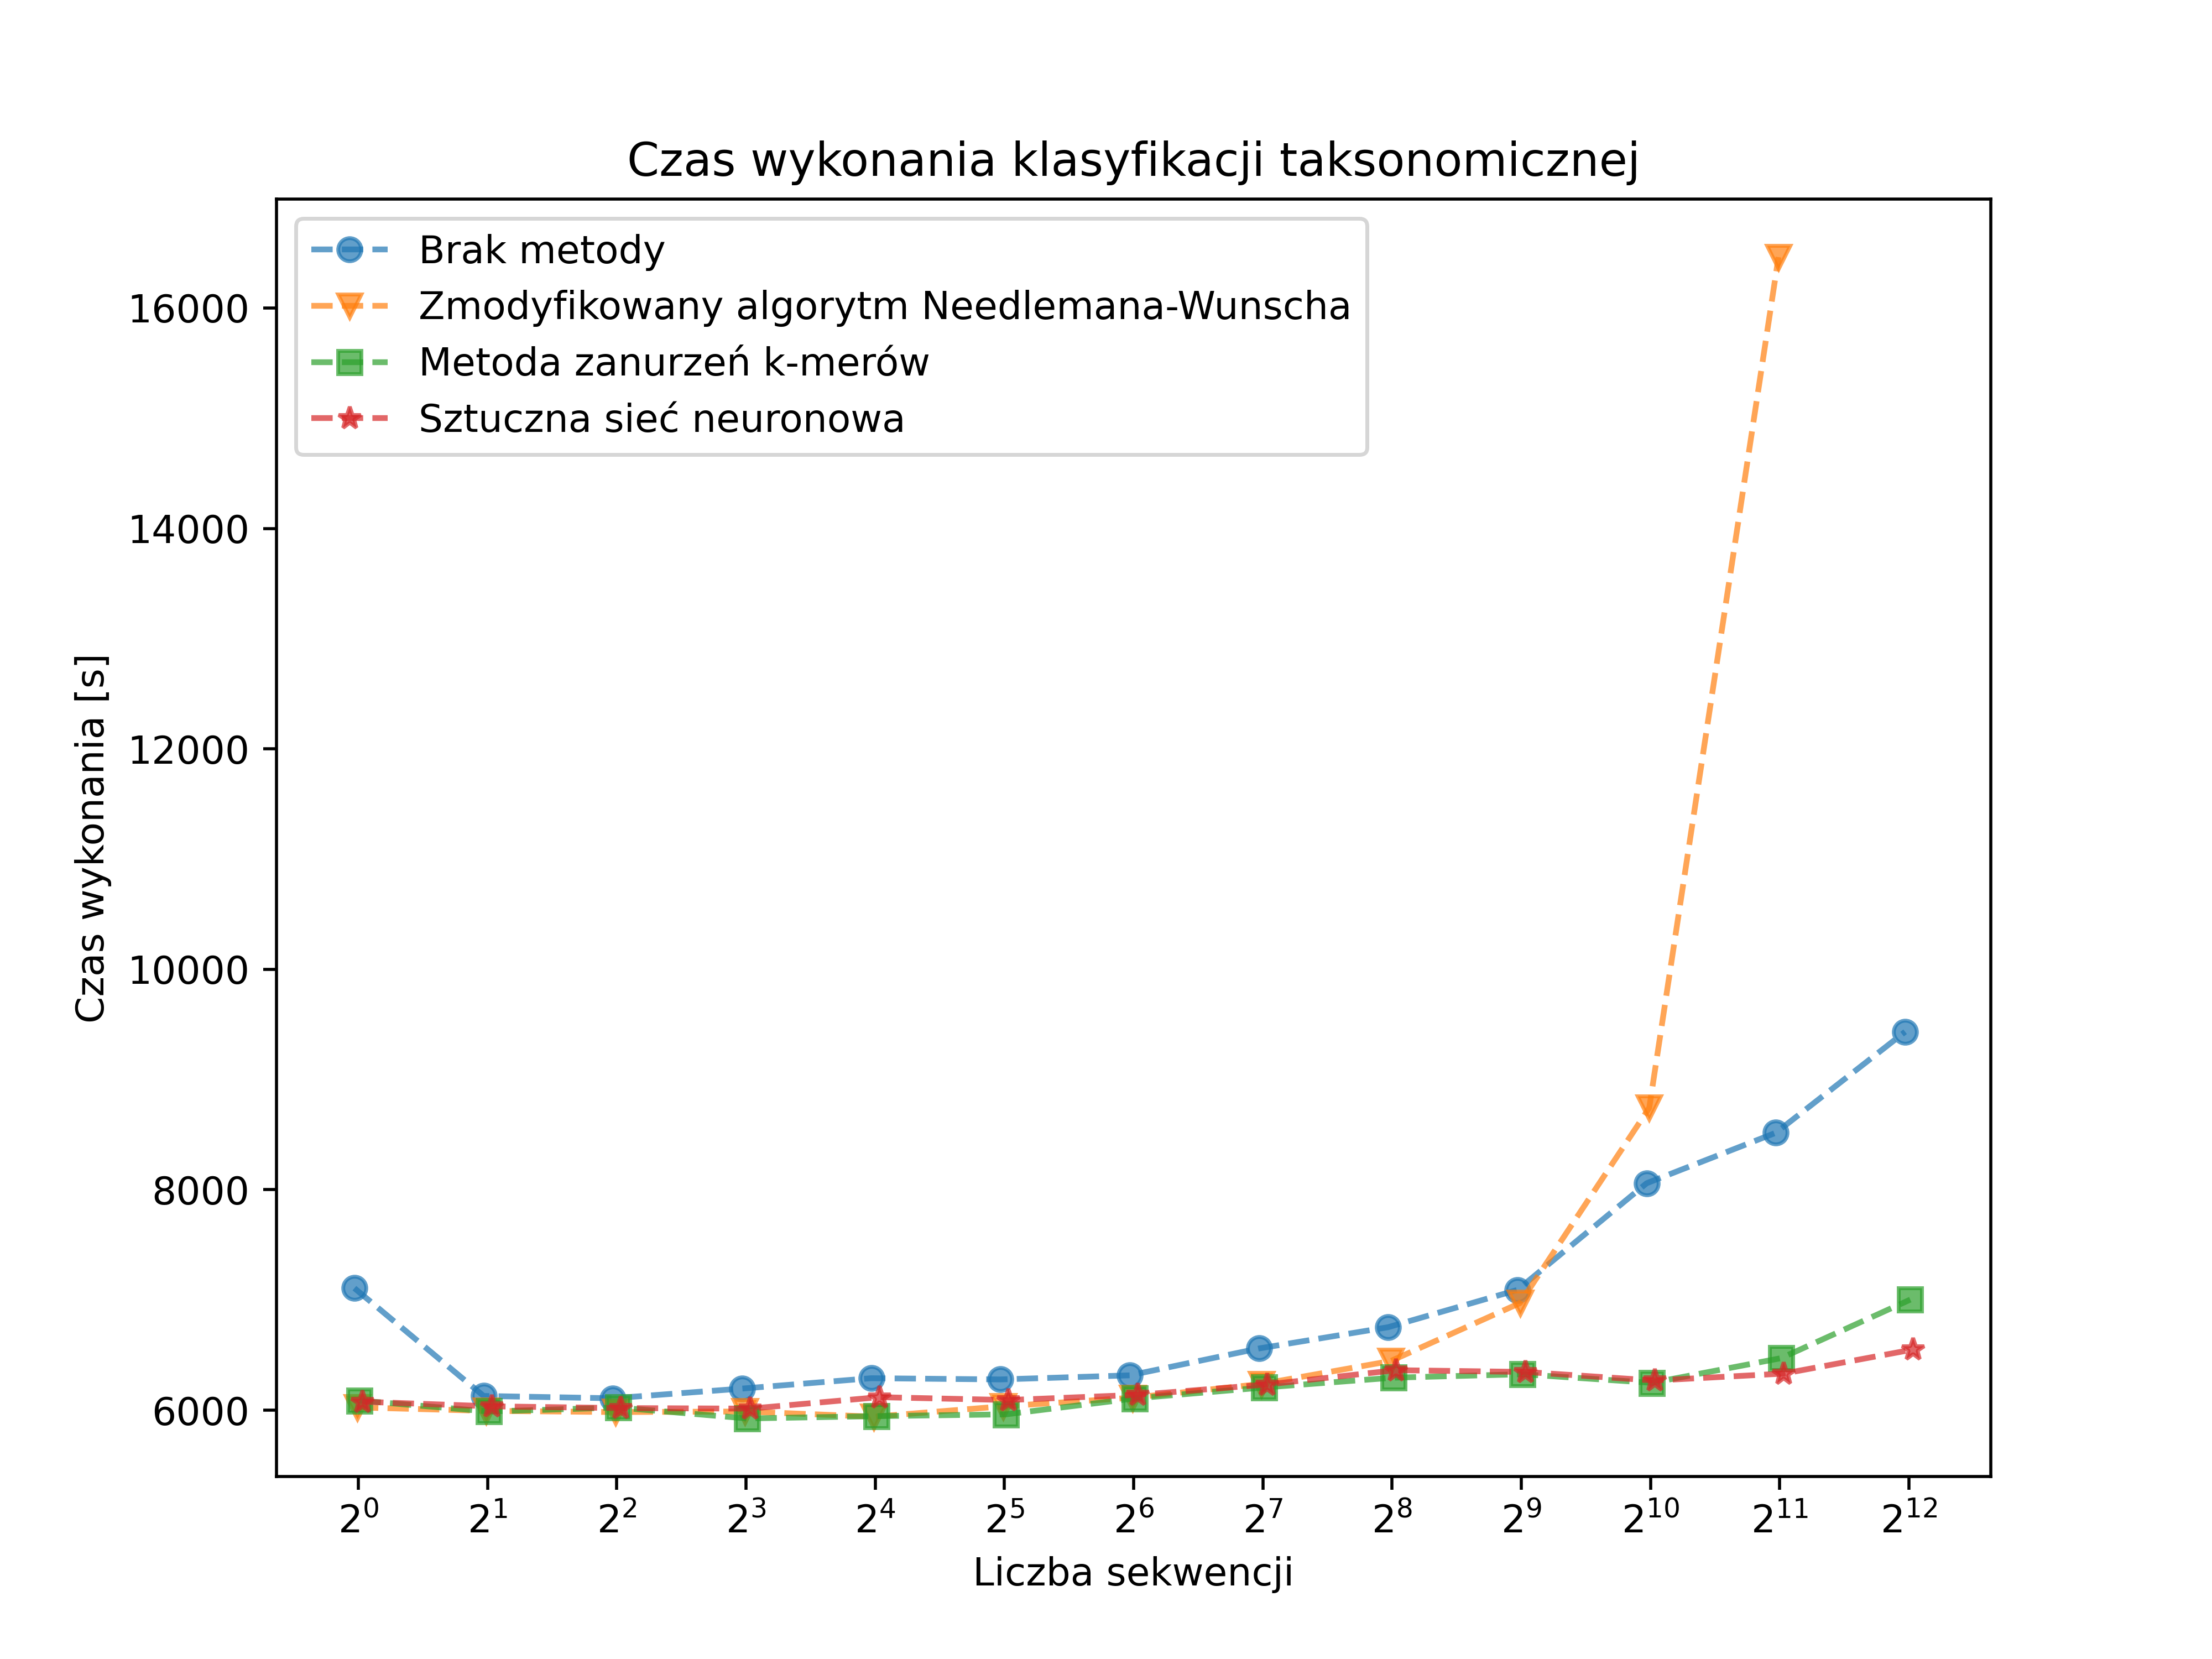
\includegraphics[width=\textwidth]{tex/pictures/exp/experiment_duration.png}
                    \end{center}
                    \caption{
                        Czas wykonania klasyfikacji taksonomicznej.
                    }\label{Picture:Experiment:Duration}
                \end{figure}

                \begin{table}\centering
                    \caption{Czas trwania eksperymentów.}\label{Table:Experiment:Duration}
                    \begin{tabularx}{\textwidth}{|c||R|R|R|R|}
                        \hline
                        \multirow{2}{*}{\textbf{Liczba sekwencji}} & \multicolumn{4}{|c|}{\textbf{Czas trwania eksperymentu}} \\ \cline{2-5}
                                        & \textbf{BZ} & \textbf{NW} & \textbf{$k$-mer} & \textbf{SSN} \\ \hline \hline
                                        1 & 7107 & \textbf{6025} & 6087 & 6077\\ \hline
                                        2 & 6129 & 5994 & \textbf{5988} & 6035\\ \hline
                                        4 & 6108 & \textbf{5983} & 6024 & 6019\\ \hline
                                        8 & 6196 & 5988 & \textbf{5925} & 6014\\ \hline
                                        16 & 6290 & \textbf{5941} & 5946 & 6118\\ \hline
                                        32 & 6279 & 6035 & \textbf{5962} & 6092\\ \hline
                                        64 & 6316 & 6113 & \textbf{6107} & 6139\\ \hline
                                        128 & 6560 & 6238 & \textbf{6206} & 6233\\ \hline
                                        256 & 6753 & 6446 & \textbf{6295} & 6363\\ \hline
                                        512 & 7091 & 6972 & \textbf{6326} & 6347\\ \hline
                                        1024 & 8059 & 8743 & \textbf{6248} & 6269\\ \hline
                                        2048 & 8517 & 16461 & 6472 & \textbf{6332}\\ \hline
                                        4096 & 9433 & \textbf{-1} & 7003 & 6550\\ \hline

                    \end{tabularx}
                \end{table}

                \begin{table}\centering
                    \caption{Wykorzystanie procesora oraz pamięci.}\label{Table:Experiment:Resources}
                    \begin{tabularx}{\textwidth}{|c||R|R|R|R||R|R|R|R|}
                        \hline
                        \multirow{2}{*}{\textbf{Liczba sekwencji}} & \multicolumn{4}{|c||}{\textbf{Wykorzystanie procesora [proc.]}} & \multicolumn{4}{|c|}{\textbf{Wykorzystanie pamięci [MB]}} \\ \cline{2-9}
                                        & \textbf{BZ} & \textbf{NW} & \textbf{$k$-mer} & \textbf{SSN} & \textbf{BZ} & \textbf{NW} & \textbf{$k$-mer} & \textbf{SSN} \\ \hline \hline
                                        1 & \textbf{14} & \textbf{14} & \textbf{14} & \textbf{14} & 37954 & 37451 & 39191 & \textbf{41120}\\ \hline
                                        2 & \textbf{15} & 14 & 14 & 14 & 37584 & 37493 & 38081 & \textbf{40567}\\ \hline
                                        4 & \textbf{16} & 14 & 14 & 14 & 37632 & 37510 & 38150 & \textbf{40701}\\ \hline
                                        8 & \textbf{18} & 14 & 15 & 13 & 37590 & 37545 & 38119 & \textbf{40685}\\ \hline
                                        16 & \textbf{22} & 15 & 16 & 17 & 37596 & 37509 & 38133 & \textbf{40781}\\ \hline
                                        32 & \textbf{21} & 15 & 16 & 15 & 37846 & 37589 & 38115 & \textbf{40766}\\ \hline
                                        64 & \textbf{21} & 17 & 17 & 17 & 37798 & 37604 & 37963 & \textbf{40706}\\ \hline
                                        128 & \textbf{26} & 21 & 20 & 19 & 37476 & 37638 & 37973 & \textbf{40396}\\ \hline
                                        256 & \textbf{32} & 25 & 22 & 20 & 37539 & 37667 & 37957 & \textbf{40385}\\ \hline
                                        512 & \textbf{38} & 33 & 25 & 23 & 37465 & 37590 & 37929 & \textbf{40414}\\ \hline
                                        1024 & \textbf{53} & 44 & 21 & 19 & 37462 & 37591 & 37876 & \textbf{40490}\\ \hline
                                        2048 & 61 & \textbf{70} & 24 & 22 & 37424 & 37607 & \textbf{37907} & 33674\\ \hline
                                        4096 & 68 & \textbf{96} & 29 & 24 & 37463 & 37504 & \textbf{37900} & 17106\\ \hline
                    \end{tabularx}
                \end{table}

            \paragraph{Wnioski}
                Metoda z wykorzystaniem zmodyfikowanego algorytmu Needlemana-Wunscha zgodnie z oczekiwaniami cechowała się najszybszym wzrostem czasu wykonania klasyfikacji taksonomicznej. Gwałtowny wzrost spowodowany jest porównywanie sekwencji każda z każdą przez budowę macierzy podobieństwa. Pomimo redukcji ilości sekwencji, które poddawane są klasyfikacji, czas wykonania tą metodą przekroczył klasyfikację taksonomiczną wszystkich sekwencji bez wykorzystania potoku przetwarzania.

                Metody z wykorzystaniem zanurzeń $k$-merów oraz sztucznej sieci neuronowej cechowały się porównywalnymi czasami wykonania z lekką przewagą dla pierwszej metody. Obie metody działały szybciej od klasyfikacji taksonomicznej bez wykorzystania potoku przetwarzania. Metody do porównywania wykorzystują reprezentacje sekwencji, co spowodowało powolniejszy wzrost czasu wykonania klasyfikacji taksonomicznej. W przypadku metody ze sztuczną siecią neuronową krótszy czas wykonania dla $4096$ sekwencji może być spowodowany obliczaniem zanurzeń dla wszystkich sekwencji jednocześnie za pomocą karty graficznej.

                W przypadku wykorzystania zasobów zauważono wzrost średniego wykorzystania procesora przez klasyfikację taksonomiczną z wykorzystaniem zaimplementowanych metod w miarę wzrostu czasu wykonania klasyfikacji, co jest związane ze znacznym nakładem obliczeniowym podczas tworzenia macierzy niepodobieństwa, której złożoność tworzenia rośnie kwadratowo wraz z liczbą sekwencji.

                Zauważalne również jest większe wykorzystanie pamięci RAM przez metodę ze sztuczną siecią neuronową, co spowodowane jest koniecznością wczytania modelu sztucznej sieci neuronowej do pamięci.

        \subsubsection{Eksperyment 2: Jakość klasyfikacji taksonomicznej}

            \paragraph{Cel}
                Celem drugiego eksperymentu było zbadanie jakości klasyfikacji taksonomicznej z wykorzystaniem zaimplementowanych metod względem klasyfikacji taksonomicznej wszystkich sekwencji. Zbadano również tworzone grupy przez zaimplementowane metody.

            \paragraph{Założenia}

                \begin{enumerate}
                    \item {
                        Proces tworzenia grup przebiega deterministycznie.
                    }
                    \item {
                        Program \texttt{BLASTn} działa deterministycznie, zwracając dla danej sekwencji i zadanych parametrów zawsze te same wyniki.
                    }
                    \item {
                        W przypadku braku możliwości obliczenia jakości dla danego przebiegu klasyfikacji taksonomicznej za wartość jakości przyjęto $0$, wartość ta nie jest brana pod uwagę w przypadku obliczania średniej jakości ważonej.
                    }
                \end{enumerate}

            \paragraph{Wyniki}
                Obliczono jakość klasyfikacji za pomocą miary wyrażonej wzorem~\ref{Equation:Quality} dla zaimplementowanych metod względem pełnej klasyfikacji taksonomicznej. Na rysunku~\ref{Picture:Experiment:Quality} przedstawiono wykres jakości klasyfikacji w zależności od ilości sekwencji wejściowych, szczegółowe wyniki jakości umieszczono w tabeli~\ref{Table:Experiment:Quality}. Średnia ważona jakość obliczona za pomocą wzoru~\ref{Equation:WeightedAverageQuality} dla metody ze zmodyfikowanym algorytmem Needlemana-Wunscha wyniosła $0,899$, dla metody z zanurzeniami $k$-merów wyniosła $0,921$, natomiast dla metody z wykorzystaniem sztucznej sieci neuronowej $0,944$. Na rysunku~\ref{Picture:Experiment:RelativeQualityNMI} przedstawiono wykres jakości względnej grup obliczony za pomocą wzoru~\ref{Equation:NMI}, natomiast na rysunku~\ref{Picture:Experiment:RelativeQualitySensitivity} przedstawiono wykres czułości obliczonej za pomocą wzoru~\ref{Equation:Sensitivity} reprezentantów grup. Szczegółowe wyniki znajdują się odpowiednio w tabeli~\ref{Table:Experiment:RelativeQualityNMI} oraz tabeli~\ref{Table:Experiment:RelativeQualitySensitivity}.

                \begin{figure}[!htb]
                    \begin{center}
                        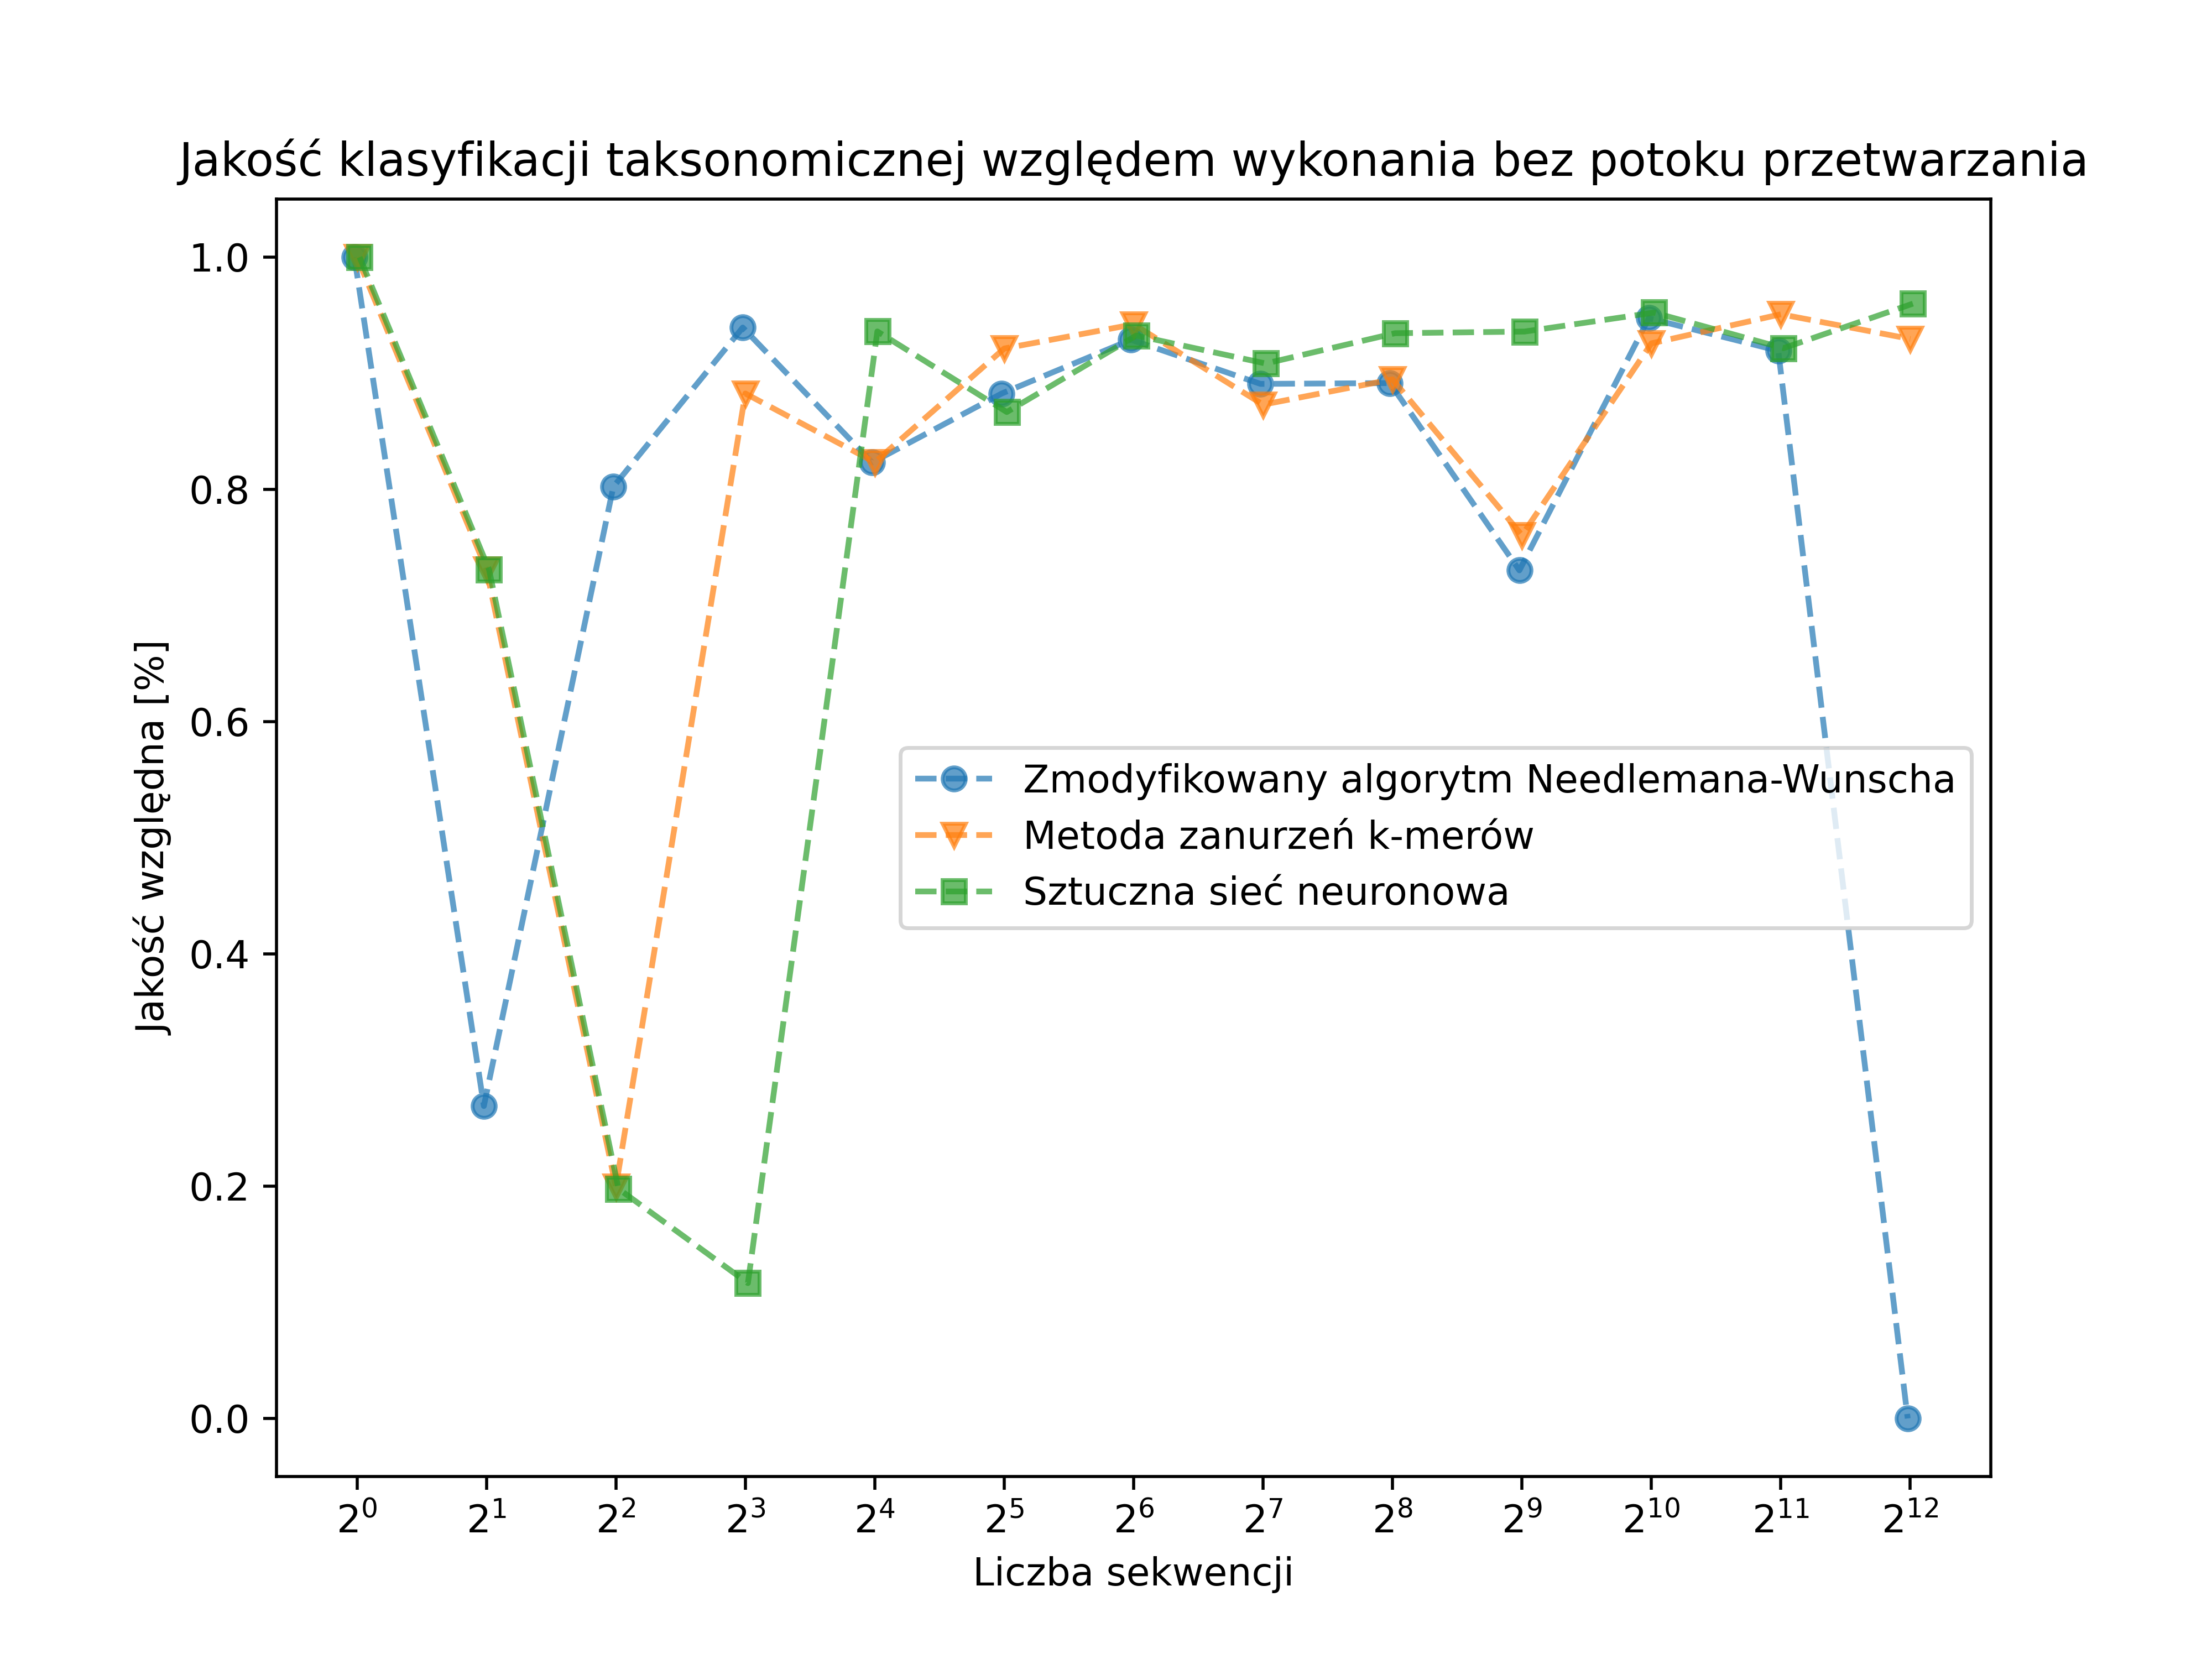
\includegraphics[width=\textwidth]{tex/pictures/exp/experiment_quality.png}
                    \end{center}
                    \caption{
                        Jakość klasyfikacji taksonomicznej.
                    }\label{Picture:Experiment:Quality}
                \end{figure}

                \begin{table}\centering
                    \caption{Jakość klasyfikacji taksonomicznej.}\label{Table:Experiment:Quality}

                    \begin{tabularx}{\textwidth}{|c|R|R|R|}
                        \hline
                        \multirow{2}{*}{\textbf{Liczba sekwencji}} & \multicolumn{3}{|c|}{\textbf{Metoda}} \\ \cline{2-4}
                        & \textbf{NW} & \textbf{$k$-mer} & \textbf{SSN} \\ \hline \hline
                        1 & \textbf{1,0} & \textbf{1,0} & \textbf{1,0}\\ \hline
                        2 & 0,27 & \textbf{0,73} & \textbf{0,73}\\ \hline
                        4 & \textbf{0,8} & 0,2 & 0,2\\ \hline
                        8 & \textbf{0,94} & 0,88 & 0,12\\ \hline
                        16 & 0,82 & 0,82 & \textbf{0,94}\\ \hline
                        32 & 0,88 & \textbf{0,92} & 0,87\\ \hline
                        64 & 0,93 & \textbf{0,94} & 0,93\\ \hline
                        128 & 0,89 & 0,87 & \textbf{0,91}\\ \hline
                        256 & 0,89 & 0,89 & \textbf{0,93}\\ \hline
                        512 & 0,73 & 0,76 & \textbf{0,94}\\ \hline
                        1024 & \textbf{0,95} & 0,93 & \textbf{0,95}\\ \hline
                        2048 & 0,92 & \textbf{0,95} & 0,92\\ \hline
                        4096 & 0,0 & 0,93 & \textbf{0,96}\\ \hline
                    \end{tabularx}
                \end{table}

                \begin{figure}[!htb]
                    \begin{center}
                        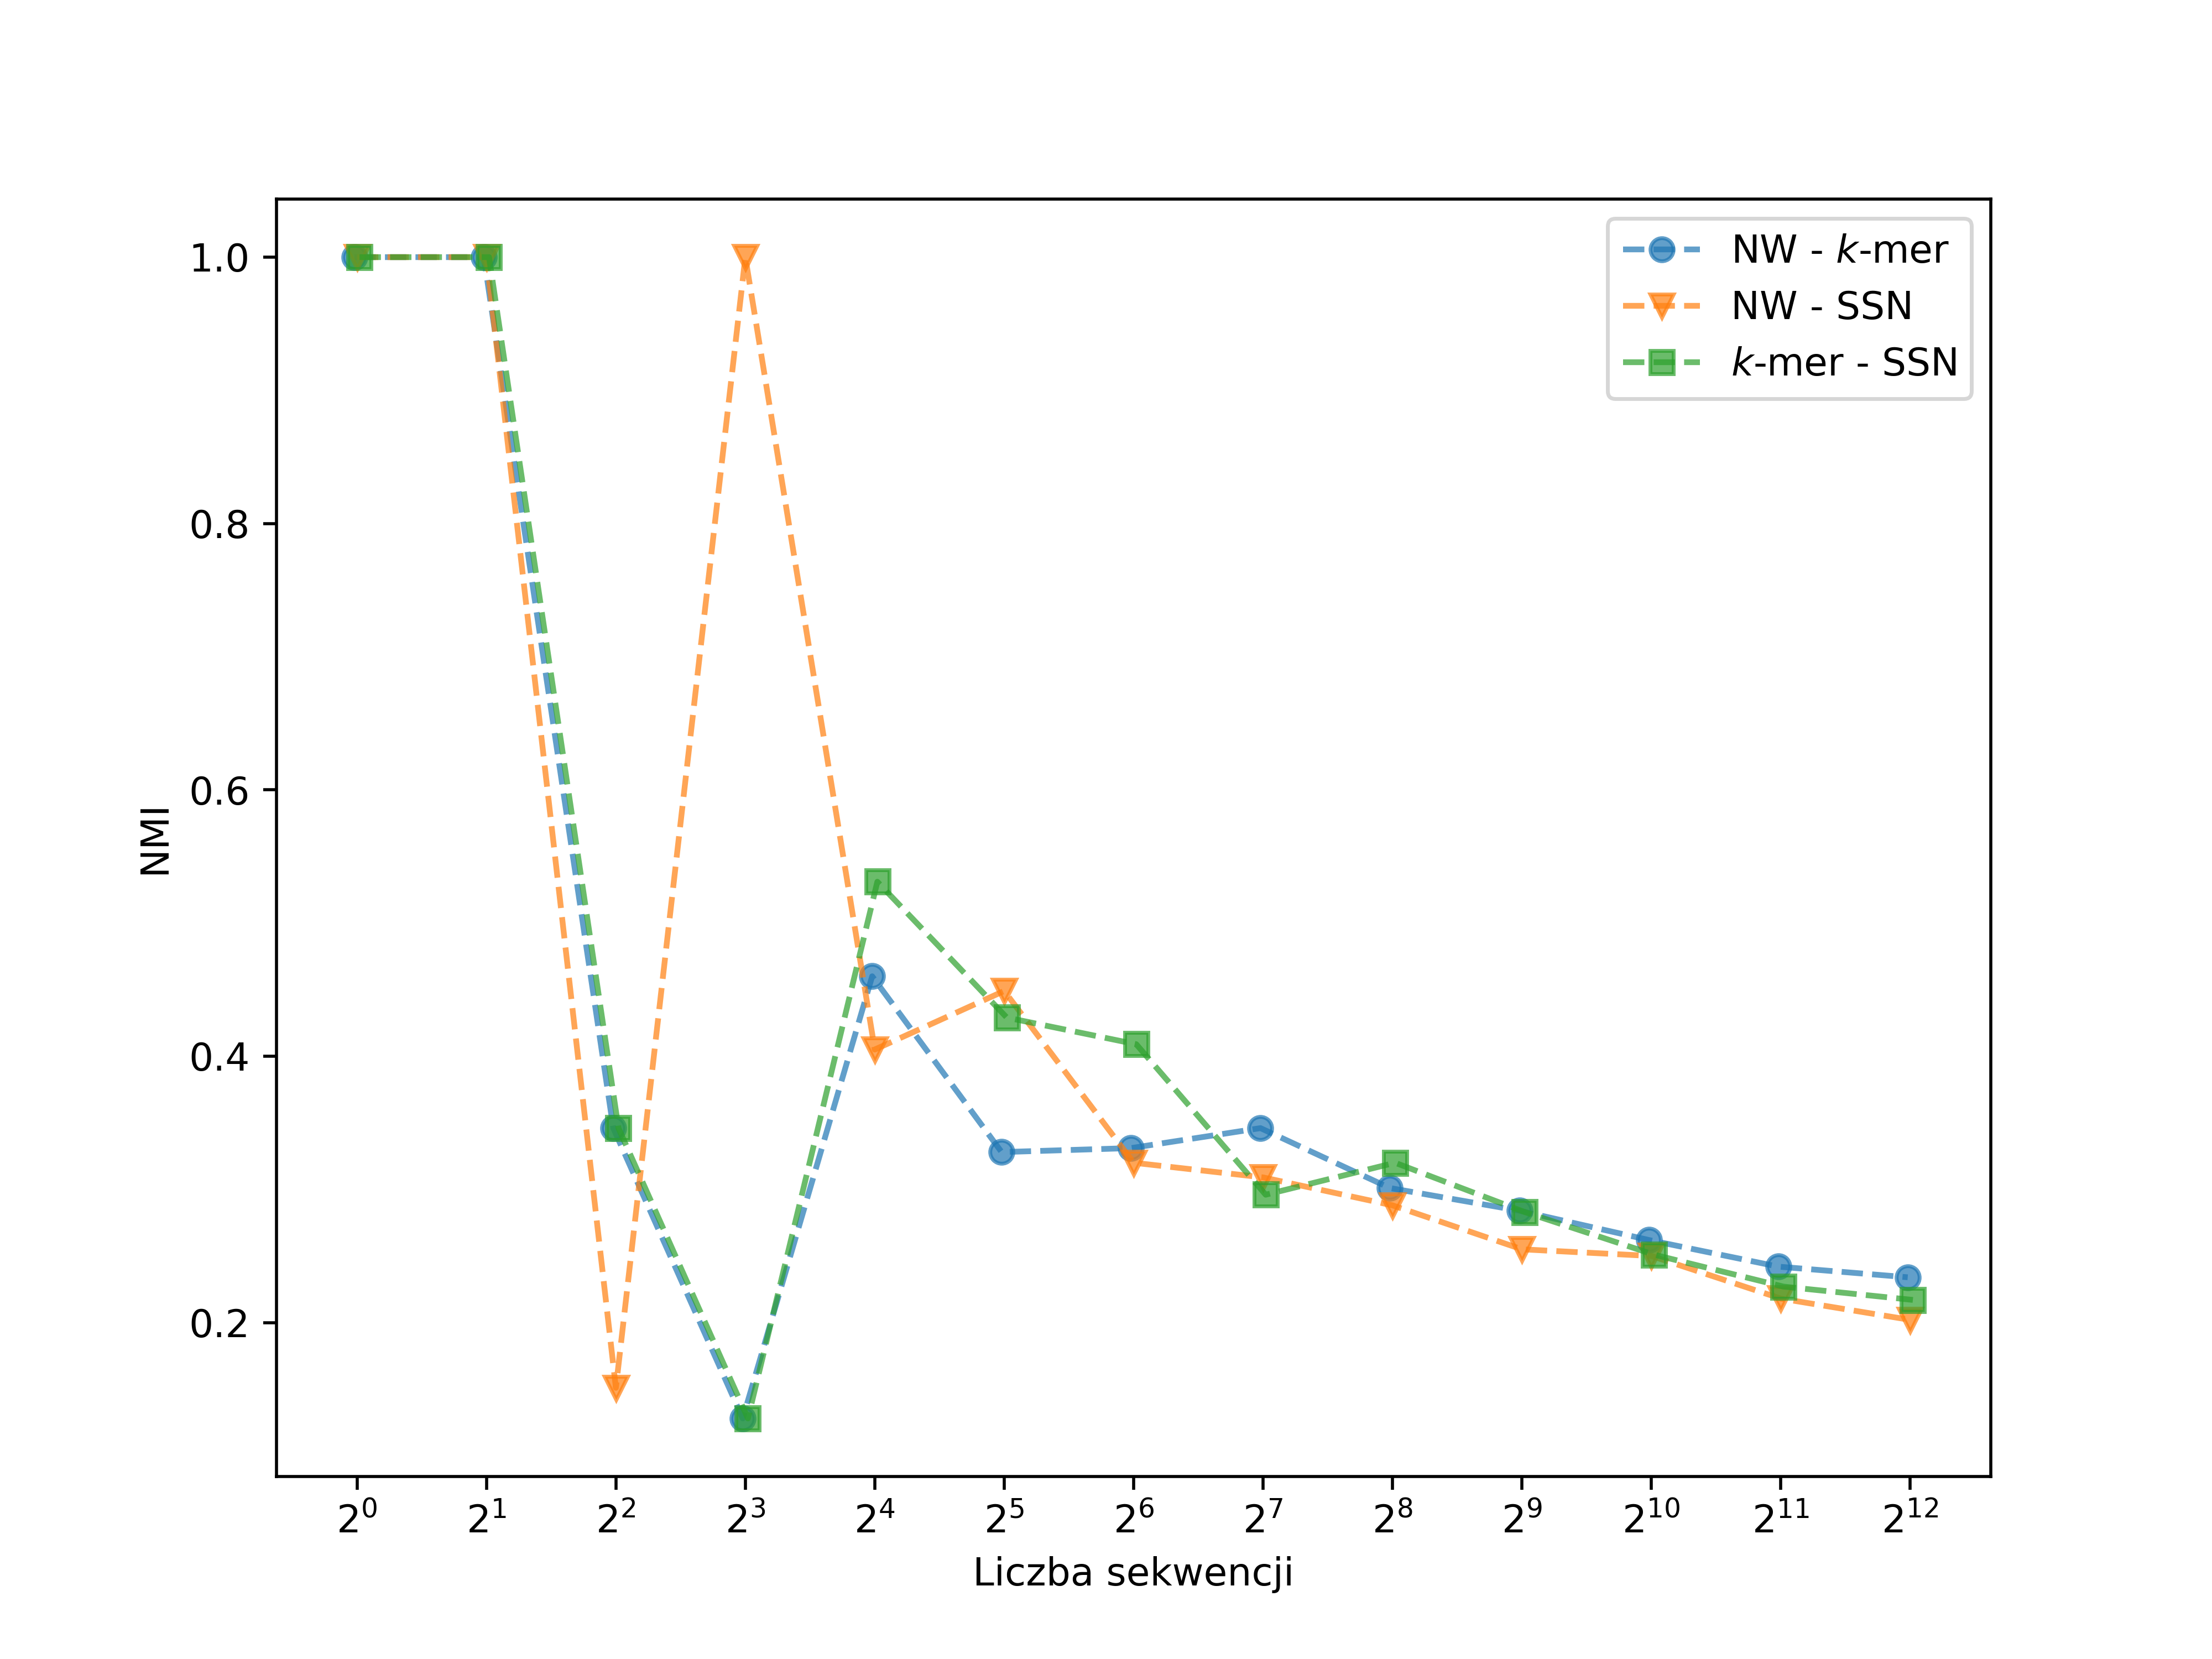
\includegraphics[width=\textwidth]{tex/pictures/exp/experiment_relative_quality_nmi.png}
                    \end{center}
                    \caption{
                       Jakość względna grup wykorzystywanych w klasyfikacji taksonomicznej.
                    }\label{Picture:Experiment:RelativeQualityNMI}
                \end{figure}

                \begin{figure}[!htb]
                    \begin{center}
                        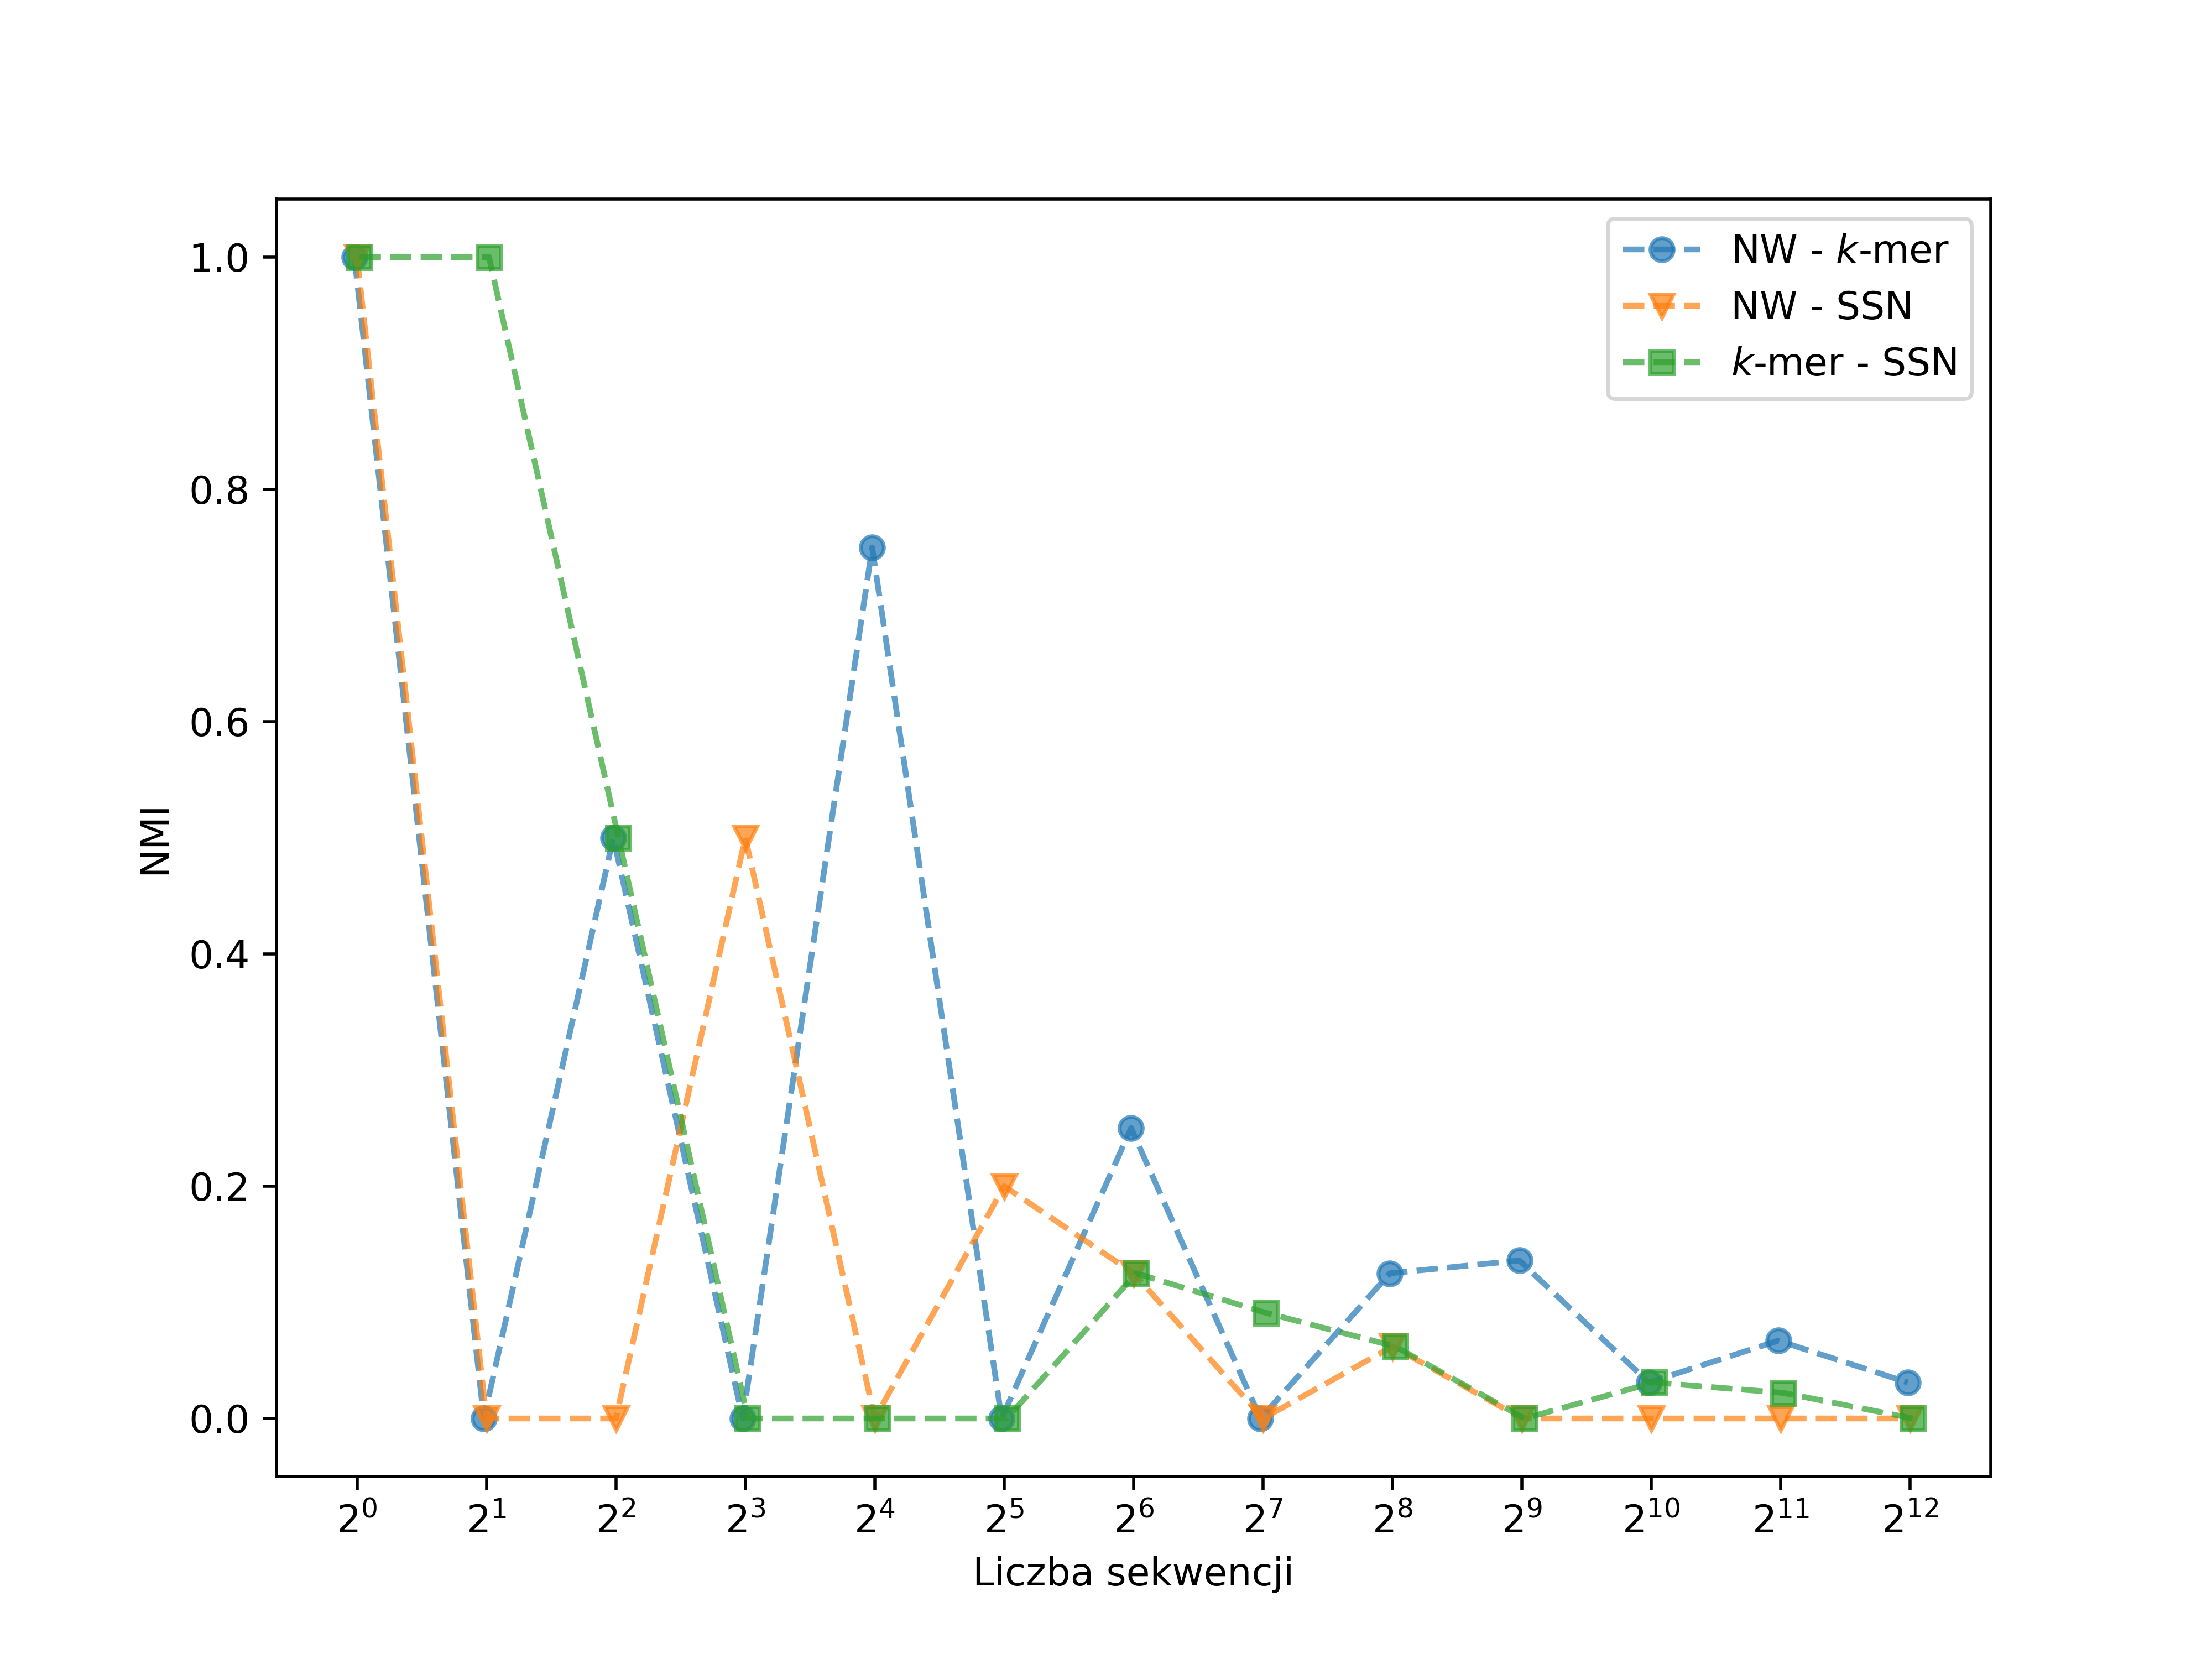
\includegraphics[width=\textwidth]{tex/pictures/exp/experiment_relative_quality_sensitivity.png}
                    \end{center}
                    \caption{
                       Czułość między reprezentantami grup wykorzystanych w klasyfikacji taksonomicznej.
                    }\label{Picture:Experiment:RelativeQualitySensitivity}
                \end{figure}

                \begin{table}\centering
                    \caption{Jakość względna grup wykorzystywanych w klasyfikacji taksonomicznej.}\label{Table:Experiment:RelativeQualityNMI}

                    \begin{tabularx}{\textwidth}{|c|R|R||R|}
                        \hline
                        \multirow{2}{*}{\textbf{Liczba sekwencji}} & \multicolumn{3}{|c|}{\textbf{Metoda}} \\ \cline{2-4}
                        & \textbf{NW - $k$-mer} & \textbf{NW - SSN} & \textbf{$k$-mer - SSN} \\ \hline \hline
                        1 & 1 & 1 & 1\\ \hline
                        2 & 1 & 1 & 1\\ \hline
                        4 & 0,346 & 0,151 & 0,346\\ \hline
                        8 & 0,128 & 1,0 & 0,128\\ \hline
                        16 & 0,46 & 0,405 & 0,531\\ \hline
                        32 & 0,328 & 0,449 & 0,429\\ \hline
                        64 & 0,331 & 0,32 & 0,409\\ \hline
                        128 & 0,346 & 0,309 & 0,296\\ \hline
                        256 & 0,301 & 0,288 & 0,32\\ \hline
                        512 & 0,284 & 0,255 & 0,283\\ \hline
                        1024 & 0,262 & 0,25 & 0,251\\ \hline
                        2048 & 0,242 & 0,218 & 0,227\\ \hline
                        4096 & 0,234 & 0,202 & 0,217\\ \hline
                    \end{tabularx}
                \end{table}

                \begin{table}\centering
                    \caption{Czułość między reprezentantami grup wykorzystanych w klasyfikacji taksonomicznej.}\label{Table:Experiment:RelativeQualitySensitivity}

                    \begin{tabularx}{\textwidth}{|c|R|R||R|}
                        \hline
                        \multirow{2}{*}{\textbf{Liczba sekwencji}} & \multicolumn{3}{|c|}{\textbf{Metoda}} \\ \cline{2-4}
                        & \textbf{NW - $k$-mer} & \textbf{NW - SSN} & \textbf{$k$-mer - SSN} \\ \hline \hline
                        1 & 1,0 & 1,0 & 1,0\\ \hline
                        2 & 0,0 & 0,0 & 1,0\\ \hline
                        4 & 0,5 & 0,0 & 0,5\\ \hline
                        8 & 0,0 & 0,5 & 0,0\\ \hline
                        16 & 0,75 & 0,0 & 0,0\\ \hline
                        32 & 0,0 & 0,2 & 0,0\\ \hline
                        64 & 0,25 & 0,125 & 0,125\\ \hline
                        128 & 0,0 & 0,0 & 0,091\\ \hline
                        256 & 0,125 & 0,062 & 0,062\\ \hline
                        512 & 0,136 & 0,0 & 0,0\\ \hline
                        1024 & 0,031 & 0,0 & 0,031\\ \hline
                        2048 & 0,067 & 0,0 & 0,022\\ \hline
                        4096 & 0,031 & 0,0 & 0,0\\ \hline
                    \end{tabularx}
                \end{table}

            \paragraph{Wnioski}
                Wszystkie zaimplementowane metody osiągnęły bardzo dobre wyniki jakości klasyfikacji, przekraczając $0,7$, w przypadkach, gdy liczba grup była znacznie większa od ilości sekwencji wejściowych. Średnia jakość ważona dla wszystkich metod również osiągnęła wysoką wartość.
                Metoda z wykorzystaniem sztucznej sieci neuronowej osiągnęła najlepszy wynik średniej jakości ważonej, wyprzedzając nieznacznie metodę z zanurzeniami $k$-merów oraz metodę ze zmodyfikowanym algorytmem Needlamana-Wunscha. Wbrew oczekiwaniom, metoda Needlemana-Wunscha osiągnęła najniższy wynik spośród zaimplementowanych metod.
                Metoda z wykorzystaniem sztucznej sieci neuronowej zawdzięcza swój wynik uwzględnieniu pełnej struktury sekwencji przez model, co pozwoliło na lepsze określenie niepodobieństwa między sekwencjami.
                Powolny spadek znormalizowanej informacji wzajemnej wraz ze wzrostem ilości sekwencji wejściowych świadczy o tworzeniu coraz mniej podobnych grup przez algorytm grupowania w wyniku zastosowania różnych metod do wyznaczania niepodobieństwa. Najbardziej podobne zbiory grup były tworzone między metodą ze zmodyfikowanym algorytmem Needlemana-Wunscha a metodą z zanurzeniami $k$-merów.

        \subsubsection{Analiza wyników}

            Wyniki eksperymentów częściowo potwierdziły oczekiwania postawione na początku badań. Wszystkie metody osiągnęły zadowalającą jakość klasyfikacji taksonomicznej. Szczególnie dobrze wypadła metoda wykorzystująca sztuczną sieć neuronową, która osiągnęła najlepszą średnią ważoną jakość klasyfikacji jednocześnie zachowując czas wykonania porównywalny z metodą opartą na zanurzeniach $k$-merów. Metoda Needlemana-Wunscha nie spełniła oczekiwań, będąc najwolniejszą metodą i osiągając wbrew oczekiwaniom jednocześnie najgorsze wyniki jakości klasyfikacji. Niska jakość klasyfikacji taksonomicznej przy małej liczbie sekwencji wejściowych może wynikać z nieodpowiedniego wyboru reprezentantów grup, co jest spowodowane zbyt małą liczbą dostępnych sekwencji. Zaimplementowane metody powinny być więc stosowane jedynie w przypadkach, gdy liczba sekwencji wejściowych przekracza pewien próg i ich wykorzystanie realnie skraca czas procesu klasyfikacji taksonomicznej. Dla badanych danych warunek ten jest osiągnięty dla $128$ sekwencji, gdzie jakość klasyfikacji taksonomicznej wynosiła nie mniej niż $0,87$, a wykorzystanie dowolnej metody grupowania skraca czas o co najmniej 5 minut, co stanowi przyśpieszenie o $5\%$ względem klasyfikacji taksonomicznej wszystkich sekwencji.
            }

    \clearpage
    \section{Discussion}

        \subsection{Interpretation of Results}

            \temporary{
                Wyniki eksperymentów częściowo potwierdziły oczekiwania postawione na początku badań. Wszystkie metody osiągnęły zadowalającą jakość klasyfikacji taksonomicznej. Szczególnie dobrze wypadła metoda wykorzystująca sztuczną sieć neuronową, która osiągnęła najlepszą średnią ważoną jakość klasyfikacji jednocześnie zachowując czas wykonania porównywalny z metodą opartą na zanurzeniach $k$-merów. Metoda Needlemana-Wunscha nie spełniła oczekiwań, będąc najwolniejszą metodą i osiągając wbrew oczekiwaniom jednocześnie najgorsze wyniki jakości klasyfikacji. Niska jakość klasyfikacji taksonomicznej przy małej liczbie sekwencji wejściowych może wynikać z nieodpowiedniego wyboru reprezentantów grup, co jest spowodowane zbyt małą liczbą dostępnych sekwencji. Zaimplementowane metody powinny być więc stosowane jedynie w przypadkach, gdy liczba sekwencji wejściowych przekracza pewien próg i ich wykorzystanie realnie skraca czas procesu klasyfikacji taksonomicznej. Dla badanych danych warunek ten jest osiągnięty dla $128$ sekwencji, gdzie jakość klasyfikacji taksonomicznej wynosiła nie mniej niż $0,87$, a wykorzystanie dowolnej metody grupowania skraca czas o co najmniej 5 minut, co stanowi przyśpieszenie o $5\%$ względem klasyfikacji taksonomicznej wszystkich sekwencji.
            }

            \temporary{
                Wykorzystanie sztucznej sieci neuronowej pozwoliło na poprawienie jakości klasyfikacji względem innych zastosowanych metod. Oprócz osiągnięcia dobrej jakości klasyfikacji nie odstaje ona od metod klasycznych.
            }

        \subsection{Limitations}

            \temporary{
                \subsubsection{Czasochłonność eksperymentów}

            Przeprowadzenie całego procesu klasyfikacji taksonomicznej sekwencji DNA z wykorzystaniem narzędzia \texttt{BLASTn} w ramach eksperymentów dla każdej metody i każdego podzbioru eksperymentalnego było procesem czasochłonnym. Łączny czas wykonania eksperymentów opisanych w pracy wyniósł około 5 dni, co spowodowało ograniczenie liczby eksperymentów do jednego przebiegu i rozmiaru podzbioru eksperymentalnego do maksymalnie $4096$ sekwencji.

        \subsubsection{Wykorzystanie jednego zbioru danych}

            W pracy wykorzystano jedynie część dostępnego zbioru danych, ograniczając się do jednej próbki ze względu na jej duży rozmiar. Wybór próbki zawierającej sekwencje DNA pochodzące z mikrobiomu skóry człowieka mógł ograniczyć przestrzeń analizowanych sekwencji, co mogło wpłynąć na wyniki eksperymentów, ponieważ w eksperymentach również wykorzystano sekwencje DNA pochodzące z tego samego mikrobiomu.
            
            subsubsection{Złożoność obliczeniowa macierzy niepodobieństwa}

            Czas budowy macierzy niepodobieństwa rośnie wprost proporcjonalnie do kwadratu liczby sekwencji, które zostały użyte do jej budowy. Macierz niepodobieństwa wykorzystywana przez algorytm grupowania w pracy była budowana dla wszystkich sekwencji wejściowych. Zastosowane podejście znacznie ogranicza liczbę możliwych sekwencji wejściowych ze względu na szybki wzrost czasu potrzebnego na tworzenie macierzy niepodobieństwa.
            }

        \subsection{Possible Improvements}

            \temporary{
                \subsubsection{Zmiana architektury modelu sztucznej sieci neuronowej}

            Stworzony model sztucznej sieci neuronowej wymaga sekwencji o stałej długości, co ogranicza elastyczność modelu w analizie sekwencji o różnych długościach i wymaga tworzenia nowego modelu dostosowanego do dłuższych sekwencji w przypadku znacznej różnicy między długościami sekwencji wejściowych a oczekiwanych przez model. Dodatkowo sekwencje krótsze niż wymagane wymagają wydłużenia do zadanej długości przez wypełnienie wybraną zasadą. W przyszłości można rozważyć zmianę architektury modelu sztucznej sieci neuronowej, dostosowując ją do analizy sekwencji o zmiennych długościach poprzez zastosowanie sieci rekurencyjnych lub typu LSTM w pierwszych warstwach modelu.

        \subsubsection{Grupowanie sekwencji w paczkach}

            Ze względu na czasochłonność procesu budowy macierzy niepodobieństwa, na wstęp\-nym etapie sekwencje wejściowe mogłyby zostać poddane losowemu grupowaniu w paczki. Następnie, w ramach każdej paczki, przeprowadzony zostałby proces wyboru reprezentantów, tak jak ma to miejsce w obecnym podejściu. Zastosowanie wstępnego grupowania umożliwiłoby ominięcie budowy jednej dużej macierzy niepodobieństwa, co pozwoliłoby na analizę większej liczby sekwencji.

        \subsubsection{Wykonywanie obliczeń równolegle}

            Możliwa jest optymalizacja niektórych operacji wykonywanych w potoku przetwarzania poprzez zastosowanie obliczeń równoległych. Pierwszym elementem, w którym można wykorzystać obliczenia równoległe, jest budowa macierzy niepodobieństwa. Macierz tą można podzielić na fragmenty, które będą budowane równolegle i niezależnie. Drugą zmianą jest modyfikacja potoku przetwarzania, która pozwalałaby na równoczesne wykonywanie niektórych etapów, bez konieczności oczekiwania na zakończenie obliczeń w innych częściach potoku. Przykładem takiego etapu jest wyliczanie zanurzeń, które mogłoby być wykorzystywane bezpośrednio do budowy macierzy niepodobieństwa bez oczekiwania na obliczenie wszystkich zanurzeń.

        \subsubsection{Automatyczny dobór liczby grup}

            Obecne podejście wymaga doboru liczby tworzonych grup przez algorytm grupowania. Liczba grup bezpośrednio determinuje liczbę reprezentantów, którzy będą poddani klasyfikacji taksonomicznej i ma wpływ na jakość oraz czas wykonania całego procesu. Możliwe byłoby zastosowanie lub stworzenie algorytmu, który automatycznie dobierałby liczbę tworzonych grup na podstawie macierzy niepodobieństwa oraz miar jakości tworzonych grup. Automatyczne dostosowanie liczby grup pozwoliłoby na zwiększenie jakości klasyfikacji w przypadku bardzo różnych sekwencji wejściowych bez spowalniania procesu dla zbiorów sekwencji bardzo podobnych.
            }

    \clearpage
    \section{Conclusions and Future Work}

        \subsection{Summary of Findings}

            \temporary{
                Stworzone rozwiązanie zostało zaimplementowane przy użyciu języka Rust, a jego struktura została odpowiednio zorganizowana w moduły, które realizują poszczególne funkcjonalności i umożliwiają łatwe rozszerzanie aplikacji. Aplikacja konsolowa pozwala w bardzo prosty sposób na uruchomienie procesu analizy oraz ustawienie wszystkich parametrów dostępnych dla zaimplementowanych metod. Aplikacja przeglądarkowa umożliwia uruchomienie analizy przy użyciu najlepszego zestawu parametrów oraz wyświetlenie wyników w czytelnej dla użytkownika postaci.

                Przeprowadzone eksperymenty wykazały, że nowa metoda oparta na sztucznych sieciach neuronowych pozwala na osiągnięcie wyższej jakości od metod klasycznych, jednocześnie zachowując czas wykonania porównywalny z metodą klasyczną wykorzystującą $k$-mery.
            }

        \subsection{Future Research Directions}

            \temporary{
                \subsubsection{Narzędzie do klasyfikacji taksonomicznej oparte o model sztucznej sieci neuronowej}

                Narzędzia do klasyfikacji taksonomicznej w większości opierają się na obliczaniu podobieństwa między sekwencjami wejściowymi a sekwencjami znajdującymi się w bazie danych sekwencji w celu znalezienia sekwencji, które są podobne. Wykorzystane w eksperymentach narzędzie \texttt{BLASTn} wykorzystuje $k$-mery do określenia podobieństwa między sekwencjami. 
                Grupowanie sekwencji, które zostało wykorzystane w pracy, wykonuje podobne operacje, do tych, które są wykonywane przez narzędzia do klasyfikacji taksonomicznej. Możliwe byłoby zatem stworzenie własnego narzędzia, które wykorzystywałoby bezpośrednio model sztucznej sieci neuronowej do określenia podobieństwa między sekwencjami i klasyfikacji taksonomicznej. Wykorzystanie sztucznych sieci neuronowych w przypadku wydajnej implementacji mogłoby pozwolić na osiągnięcie akceptowalnego czasu działania przy wyższej jakości.
            }

\end{document}